\documentclass[11pt,a4paper]{report}

\usepackage[margin=1in]{geometry}
\usepackage[T1]{fontenc}
\usepackage{indentfirst}
\usepackage{amsmath,amssymb,amsthm}
\usepackage{booktabs}
\usepackage{longtable}
\usepackage{hyperref}
\usepackage{enumitem}
\usepackage{graphicx}
\usepackage{subcaption}
\usepackage{tabularx}
\usepackage{array}

\setlength{\parindent}{1.5em}
\setlength{\parskip}{0.3em}

\hypersetup{
    colorlinks=true,
    linkcolor=blue,
    citecolor=blue,
    urlcolor=blue
}

\title{The Tempered Fractional Black--Scholes Model as a Diagnostic Pricing Framework: Cross-Asset Evidence Across Option Maturities}
\author{Useong Jeong}
\date{June 15, 2026}

\begin{document}

\maketitle
\newpage

\chapter*{Abstract}
\addcontentsline{toc}{chapter}{Abstract}

This thesis introduces the Tempered Fractional Black--Scholes (TFBS) model in order to extend the memory-free structure of the classical Black--Scholes model, and examines whether the model can produce lower validation pricing errors than the Black--Scholes benchmark on observed option price data. The Black--Scholes model is a canonical benchmark in option pricing theory, but because it assumes constant volatility and a Markovian structure, it cannot directly represent non-local time dependence or memory effects that may be embedded in option prices. To address this limitation, this thesis considers a TFBS model in which the classical time derivative in the Black--Scholes PDE is replaced by a tempered Caputo fractional derivative. In this formulation, the fractional order $\alpha$ controls the shape of the memory kernel, while the tempering parameter $\lambda$ controls the rate at which the influence of past information decays with the time lag.

The empirical analysis uses call option chains on major U.S. equities and ETFs. For each maturity, the option chain is split into a calibration set and a validation set. Model parameters estimated from the calibration set are then applied to validation strikes that were not used in calibration, and the resulting pricing error is measured. Validation RMSE is used as the main comparison criterion. Maturities are divided into short, medium, and long maturity buckets in order to examine whether TFBS performance is more pronounced in specific maturity ranges. The underlying assets are also grouped into liquid blue-chip equities, high-attention or event-driven equities, and commodity-linked ETFs, so that the dependence of TFBS performance on asset characteristics can be examined.

The results show that the TFBS model does not uniformly improve upon the Black--Scholes benchmark across all assets and maturities. Some assets exhibit lower validation RMSE in the medium or long maturity bucket, while others show weak or negative improvement. In particular, AMZN displays a clear improvement in the medium maturity bucket, whereas MSFT and several high-attention assets do not translate the additional flexibility of TFBS into better validation performance. These findings indicate that TFBS performance is not universal, but is both maturity-dependent and asset-specific. Accordingly, this thesis interprets the TFBS model not as a universal replacement for Black--Scholes, but as a reduced-form diagnostic pricing model for detecting whether a finite-horizon memory-tempering structure is present in an option surface.

\newpage
\tableofcontents

\chapter{Introduction}

\section{Motivation}

The Black--Scholes model has long served as the most basic benchmark model in option pricing theory. Under the assumption that the underlying asset price follows geometric Brownian motion, the model provides a closed-form price for European options and has become the starting point for most subsequent option pricing models \cite{BlackScholes1973,Merton1973}. In real financial markets, however, several empirical phenomena are difficult to explain using the simple assumptions of Black--Scholes. In particular, implied volatility varies across strike prices and maturities, producing volatility smiles, skews, and term structures \cite{Dupire1994,DumasFlemingWhaley1998,Gatheral2006}. Asset returns also exhibit stylized facts such as volatility clustering and long-range dependence \cite{Cont2001}. Moreover, rough volatility has been studied as a framework that goes beyond classical Markovian descriptions of volatility and captures non-local temporal structure \cite{GatheralJaissonRosenbaum2018}.

These phenomena suggest that option prices are not fully explained by the current underlying price, strike, maturity, interest rate, and a constant volatility alone. In the Black--Scholes framework, once the current underlying price and fixed parameters are given, the past price path does not appear as an explicit state variable in the pricing equation. If the option surface reflects the influence of past information or non-local time dependence, it is therefore natural to consider extensions of the classical time derivative.

One way to incorporate such memory effects mathematically is to replace the classical first-order time derivative with a fractional derivative. A fractional derivative makes the current rate of change depend on a weighted average of past rates of change, thereby introducing a time-nonlocal structure into the model \cite{Podlubny1999}. The initial direction of this study was to analyze option-price memory effects using the Fractional Black--Scholes (FBS) model, in which the time derivative of the Black--Scholes PDE is replaced by a Caputo fractional derivative \cite{Wyss2000, CarteaDelCastilloNegrete2007}.

Preliminary experiments in this study, however, showed that the basic FBS model can be unstable when applied to observed option chains, especially for short maturities. In particular, estimates of the fractional order were unstable and pricing errors fluctuated substantially. Because the Caputo memory kernel in the basic FBS model decays as a power law, the single fractional order $\alpha$ must simultaneously describe both the shape of the memory kernel and the persistence of the memory effect. This motivates an additional structure in which past information may affect option prices while its influence gradually weakens within a finite horizon.

For this reason, this thesis focuses on the Tempered Fractional Black--Scholes (TFBS) model. The TFBS model introduces exponential tempering into the Caputo fractional derivative and separates fractional memory structure from memory decay \cite{SabzikarMeerschaertChen2015}. The fractional order $\alpha$ describes the shape of the memory kernel, while the tempering parameter $\lambda$ controls how quickly the influence of past information decays with the time lag. Thus, TFBS can be interpreted as an extended fractional PDE model that complements the untempered power-law memory structure of the basic FBS model while allowing for finite-horizon memory effects.

\section{Research Question}

The central research question of this thesis is the following.

\begin{quote}
Can the Tempered Fractional Black--Scholes model reduce validation pricing error relative to the classical Black--Scholes model?
\end{quote}

Because the TFBS model contains more parameters than the Black--Scholes model, it may naturally produce lower in-sample errors on calibration data. For this reason, the comparison in this thesis is based not on calibration error, but on validation pricing error for strikes that are not used in calibration. For each maturity, the option chain is split into a calibration set and a validation set. Model parameters are estimated on the calibration set and predictive performance is evaluated on the validation set.

The thesis also focuses on maturity-dependent performance. Options are divided into short, medium, and long maturity buckets, and the validation RMSE of the Black--Scholes model and the TFBS model is compared within each bucket. The baseline maturity classification used in this thesis is

\begin{align*}
\text{Short maturity} &: \quad T \leq 30 \text{ days}, \\
\text{Medium maturity} &: \quad 30 < T \leq 180 \text{ days}, \\
\text{Long maturity} &: \quad T > 180 \text{ days}.
\end{align*}

This design makes it possible to determine whether any advantage of the TFBS model appears uniformly across all maturities or only in specific maturity ranges. Finally, the thesis studies asset-dependent performance. The same TFBS structure may perform differently depending on the nature of the underlying asset. The assets are grouped into three broad categories. The first group consists of liquid blue-chip equities such as AAPL, MSFT, GOOGL, AMZN, and JPM. The second group consists of high-attention or event-driven equities such as TSLA, GME, and DJT. The third group consists of commodity or spot-linked ETFs such as GLD and USO. This classification helps determine whether the improvement of TFBS depends not only on maturity structure, but also on whether the option surface of an asset exhibits a stable memory-tempering structure.

\section{Main Idea}

The Black--Scholes model is used in this thesis as the memory-free benchmark \cite{BlackScholes1973,Merton1973}. It determines option prices from the current underlying price, strike, maturity, interest rate, and volatility, and it uses a classical first-order derivative in the time direction. Consequently, in the Black--Scholes framework, the past price path does not enter the pricing equation as an explicit state variable once the current underlying price and fixed parameters are given.

A natural first extension is to replace the time derivative in the Black--Scholes PDE with a Caputo fractional derivative \cite{Podlubny1999,Wyss2000}. This leads to the Fractional Black--Scholes (FBS) model. In the FBS model, the fractional order $\alpha$ is the key parameter representing memory effects. However, because the Caputo memory kernel decays as a power law, the single parameter $\alpha$ must describe both the shape of the memory kernel and the persistence of the memory. In other words, the FBS model introduces memory, but does not provide a separate parameter that controls how quickly that memory decays.

This thesis therefore focuses on the Tempered Fractional Black--Scholes (TFBS) model. The TFBS model introduces exponential tempering into the Caputo fractional derivative, so that the memory kernel can be interpreted as \cite{SabzikarMeerschaertChen2015}
\[
K_{\alpha,\lambda}(t)
=
e^{-\lambda t}t^{-\alpha}.
\]

Here $\alpha$ represents the shape of the fractional memory kernel, and $\lambda$ controls the decay rate of the memory effect. Thus, the TFBS model separates memory structure from memory decay. In particular, when $\lambda=0$, the tempered kernel becomes the ordinary Caputo kernel, so TFBS is a natural extension of FBS.

The main empirical analysis compares the validation performance of the Black--Scholes model and the TFBS model. Because the TFBS model includes more parameters than Black--Scholes, comparing calibration errors alone would not distinguish genuine predictive improvement from in-sample fitting due to additional flexibility. Therefore, this thesis splits each option chain by maturity into calibration and validation sets. Parameters estimated from calibration strikes are applied to validation strikes, and out-of-sample pricing error is computed. The primary comparison criterion is validation RMSE.

The thesis further examines whether TFBS performance varies with maturity and asset characteristics. Options are divided into short, medium, and long maturity buckets, and the reduction in validation RMSE relative to the Black--Scholes benchmark is measured in each bucket. Medium maturity options may be less affected by microstructure noise and payoff nonlinearity near expiration than short maturity options, while also being less dominated by long-run macro or structural uncertainty than long maturity options. For this reason, the thesis examines whether the memory-tempering structure of TFBS appears more clearly in medium maturity options.

\section{Contributions}

This thesis makes three main contributions.

First, it organizes the Black--Scholes PDE, the FBS PDE, and the TFBS PDE within a unified fractional PDE framework. In particular, it introduces the Caputo fractional derivative and the tempered Caputo fractional derivative, and interprets $\alpha$ and $\lambda$ as parameters governing memory structure and memory decay, respectively. This shows that TFBS is not merely an ad hoc model with one additional parameter, but a natural extension that complements the untempered memory structure of FBS.

Second, the thesis constructs a numerical scheme and calibration--validation framework for the TFBS PDE. The tempered Caputo derivative is discretized in the time direction using an L1-type scheme, and the spatial direction is treated with a finite difference method \cite{SabzikarMeerschaertChen2015,ZhouGuZhaoLi2024}. The fully discrete problem reduces to a tridiagonal linear system at each time step. For option data, calibration strikes and validation strikes are separated by maturity, and the Black--Scholes and TFBS models are compared using validation RMSE. This design is intended to reduce the risk of interpreting simple in-sample overfitting as model improvement.

Third, the thesis empirically analyzes the maturity-dependent and asset-specific performance of the TFBS model. The underlying assets are divided into liquid blue-chip equities, high-attention or event-driven equities, and commodity or spot-linked ETFs. For each asset, validation pricing errors are compared by maturity bucket. The results show that TFBS improvement is not automatically determined by a particular asset class or maturity range, but depends on the memory-tempering signature of each option surface.

\section{Organization of the Thesis}

The remainder of the thesis is organized as follows. Chapter 2 reviews the classical Black--Scholes model and its limitations. Chapter 3 introduces the fractional-calculus concepts required for the analysis, including the Riemann--Liouville fractional integral, the Caputo fractional derivative, and the tempered Caputo derivative. Chapter 4 defines the FBS and TFBS models, discusses the limitations of the untempered FBS memory structure, and presents the TFBS model as an extension.

Chapter 5 presents the finite difference scheme and the calibration--validation methodology for the TFBS PDE. It explains the L1 discretization of the tempered Caputo derivative, the spatial finite difference approximation, and the tridiagonal linear system that arises at each time step. Chapter 6 describes the experimental design, including option data, asset classification, maturity buckets, and parameter grids.

Chapter 7 reports the empirical results. It compares liquid blue-chip equities, high-attention or event-driven equities, and commodity or spot-linked ETFs, and examines how much the TFBS model reduces validation RMSE relative to the Black--Scholes benchmark for each asset and maturity bucket. Chapter 8 discusses candidate drivers of asset-dependent performance, including finite-horizon memory structure, short-maturity noise, option-surface smoothness, event-driven instability, and commodity or macro factors. Chapter 9 summarizes robustness issues and model limitations, including grid sensitivity, price source, numerical resolution, maturity bucket definitions, and the calibration--validation split. Chapter 10 concludes by summarizing the main findings, limitations, and directions for future research.

\chapter{Classical Black--Scholes Model and Its Limitations}

\section{The Black--Scholes Framework}

The Black--Scholes model is one of the most fundamental benchmark models in option pricing theory \cite{BlackScholes1973,Merton1973}. Its central assumption is that the underlying asset price evolves as a continuous-time stochastic process whose dynamics are given by geometric Brownian motion. If $S_t$ denotes the underlying asset price, then under the physical measure the price process is commonly written as
\[
dS_t = \mu S_t\,dt + \sigma S_t\,dW_t,
\]
where $\mu$ is the expected return of the underlying asset, $\sigma>0$ is constant volatility, and $W_t$ is a standard Brownian motion. The risk-free asset $B_t$ is assumed to satisfy
\[
dB_t = rB_t\,dt,
\]
where $r$ is the risk-free interest rate.

In option pricing, the dynamics under the risk-neutral measure are more important than the physical drift $\mu$. If $q$ denotes the continuous dividend yield, then under the risk-neutral measure $\mathbb{Q}$ the underlying asset follows
\[
dS_t = (r-q)S_t\,dt + \sigma S_t\,dW_t^{\mathbb{Q}}.
\]
Thus, in the Black--Scholes model, an option price is determined by the current underlying price, strike, maturity, interest rate, dividend yield, and constant volatility $\sigma$. The volatility $\sigma$ is assumed to be independent of both time and the price level.

In this thesis, the Black--Scholes model is used as the benchmark against which the fractional models are compared. In particular, when evaluating TFBS performance, the Black--Scholes volatility parameter is calibrated separately for each maturity of the option chain, and pricing errors are compared on validation strikes.

\section{Derivation of the Black--Scholes PDE}

Let $V(S,t)$ be the price of a European option written on the underlying asset. Assuming that $V$ is sufficiently smooth, Ito's lemma gives
\[
dV
=
\left(
V_t
+
(r-q)S V_S
+
\frac{1}{2}\sigma^2 S^2 V_{SS}
\right)dt
+
\sigma S V_S\,dW_t^{\mathbb{Q}}.
\]
By the no-arbitrage principle, or equivalently by the risk-neutral pricing argument, the option price satisfies the Black--Scholes PDE \cite{BlackScholes1973,Merton1973}
\[
V_t
+
\frac{1}{2}\sigma^2 S^2 V_{SS}
+
(r-q)S V_S
-
rV
=
0.
\]
Here $V_t$ is the derivative with respect to time $t$, while $V_S$ and $V_{SS}$ are the first and second derivatives with respect to the underlying price $S$.

For the finite difference scheme used later in this thesis, it is convenient to work with time to maturity,
\[
\tau = T-t.
\]
Writing $C(S,\tau)=V(S,T-\tau)$, the point $\tau=0$ corresponds to the option maturity, and larger $\tau$ means a longer remaining time to maturity. Under this change of variables, the Black--Scholes PDE can be written as
\[
\frac{\partial C}{\partial \tau}
=
\mathcal{L}_{BS} C,
\]
where
\[
\mathcal{L}_{BS} C
=
\frac{1}{2}\sigma^2 S^2 C_{SS}
+
(r-q)S C_S
-
rC.
\]
The operator $\mathcal{L}_{BS}$ is the Black--Scholes spatial operator. The FBS and TFBS models are obtained by replacing the classical first-order time derivative on the left-hand side with a fractional or tempered fractional derivative.

\section{Terminal and Boundary Conditions for Call Options}

The payoff of a European call option at maturity is
\[
C(S,0) = (S-K)^+,
\]
where $K$ is the strike price and $(x)^+=\max(x,0)$. In the time-to-maturity formulation, this payoff is used as the initial condition.

The spatial boundary conditions are set as follows. If the underlying price is zero, the call option cannot be exercised, so
\[
C(0,\tau)=0.
\]
When $S$ is sufficiently large, the call option is deep in-the-money and its price is close to the forward-adjusted intrinsic value. Therefore, for a large value $S_{\max}$, the upper boundary condition is taken to be
\[
C(S_{\max},\tau)
\approx
S_{\max}e^{-q\tau}
-
Ke^{-r\tau}.
\]
Since a numerical scheme cannot directly handle the infinite spatial domain $S\in[0,\infty)$, a sufficiently large $S_{\max}$ is chosen and the finite difference method is applied on $[0,S_{\max}]$. The TFBS numerical scheme in this thesis uses the same payoff and boundary conditions.

\section{Closed-Form Black--Scholes Formula}

For a European call option, the Black--Scholes PDE admits a closed-form solution \cite{BlackScholes1973,Merton1973}. Let $S_0$ be the current underlying price, $T$ the time to maturity, and $K$ the strike. With continuous dividend yield $q$, the Black--Scholes call price is
\[
C_{BS}(S_0,K,T,r,q,\sigma)
=
S_0 e^{-qT}N(d_1)
-
K e^{-rT}N(d_2),
\]
where
\[
d_1
=
\frac{
\log(S_0/K)
+
(r-q+\frac{1}{2}\sigma^2)T
}{
\sigma\sqrt{T}
},
\qquad
d_2=d_1-\sigma\sqrt{T}.
\]
Here $N(\cdot)$ denotes the cumulative distribution function of the standard normal distribution. Setting $q=0$ gives the commonly used Black--Scholes formula for non-dividend-paying stocks.

In this thesis, the Black--Scholes model is used as a benchmark that calibrates one volatility parameter $\sigma$ for each maturity. For maturity $T_j$, the value $\sigma_j$ is chosen to minimize the squared error between observed option prices and Black--Scholes prices. The pricing error is then computed on validation strikes of the same maturity and compared with the validation error of the TFBS model.

\section{Limitations of the Classical Black--Scholes Model}

The Black--Scholes model is important because it is mathematically simple and provides a benchmark for option pricing. However, it has several limitations when applied to real market data.

\subsection{Constant Volatility Assumption}

In the Black--Scholes model, volatility $\sigma$ is assumed to be constant. In observed option markets, however, implied volatility often varies across strikes and maturities. That is, markets display volatility smiles, volatility skews, and volatility term structures \cite{Dupire1994,Heston1993,DumasFlemingWhaley1998,Gatheral2006}. This means that a single constant $\sigma$ cannot fully explain option prices across all strikes and maturities. Stochastic-volatility, local-volatility, and implied-volatility-function approaches were developed precisely to address these empirical deviations from the constant-volatility benchmark \cite{Heston1993,Dupire1994,DumasFlemingWhaley1998}.

This thesis calibrates Black--Scholes volatility separately for each maturity in order to make the benchmark as fair as possible. Even then, the benchmark cannot fully capture the strike-wise volatility smile within a given maturity. This limitation is important because the empirical object being fitted is not a single option price, but a cross-section of option prices that can be equivalently viewed as part of an implied volatility surface \cite{Gatheral2006}.

\subsection{Markovian and Memory-Free Structure}

Another important feature of the Black--Scholes model is its Markovian structure. Once the current underlying price is given, the past price path has no direct influence on future dynamics. In real financial markets, however, phenomena such as long-range dependence suggest that past market information may affect current price formation \cite{MandelbrotVanNess1968,ComteRenault1998}. Rough volatility is distinct from long memory, but it also provides a non-local volatility framework beyond classical Markovian volatility descriptions \cite{GatheralJaissonRosenbaum2018}. Such features may be reflected in option prices. Therefore, the memory-free structure of Black--Scholes may be insufficient for describing non-local time dependence in option surfaces.

\section{Motivation for Fractional Time Dynamics}

The limitations above motivate extensions of the Black--Scholes model. A natural approach for incorporating memory effects in the time direction is to replace the classical first-order derivative with a fractional derivative. The Caputo fractional derivative is a weighted average of the past rates of change of a function, and therefore allows the model to include a structure in which the option price depends non-locally on past information \cite{Podlubny1999,Caputo1967}.

The simplest extension is the FBS model, in which the time derivative of the Black--Scholes PDE is replaced by a Caputo fractional derivative \cite{Wyss2000,Magdziarz2009,CarteaDelCastilloNegrete2007}. However, the memory kernel in the basic FBS model decays as a power law, so the single fractional order $\alpha$ must describe both the shape of the memory kernel and the persistence of the memory effect. To control memory structure and memory decay separately, an additional parameter is needed.

For this reason, this thesis focuses on the TFBS model with an exponentially tempered Caputo derivative \cite{SabzikarMeerschaertChen2015}. In the TFBS model, $\alpha$ represents the fractional shape of the memory kernel, while $\lambda$ controls the exponential decay of the memory effect. Thus, TFBS can be viewed as an intermediate extension between the memory-free Black--Scholes model and the untempered long-memory FBS model, allowing finite-horizon memory to be represented.

The next chapter introduces the Riemann--Liouville fractional integral, the Caputo fractional derivative, and the tempered Caputo derivative in order to define these fractional time dynamics more precisely.

\chapter{Fractional Calculus Preliminaries}

\section{Motivation for Fractional Operators}

In classical calculus, differentiation is defined for integer orders. For example, the first-order derivative represents the instantaneous rate of change of a function, and the time direction in the Black--Scholes PDE is also described by a classical first-order derivative. Such a local derivative uses only information near the current time. It is therefore limited in its ability to represent memory effects in which the entire past path influences the current state.

Fractional calculus extends differentiation and integration from integer orders to non-integer real orders \cite{Podlubny1999}. Unlike an ordinary derivative, a fractional derivative is a non-local operator. A fractional derivative at a given time depends not only on the local rate of change at that time, but also on past function values or past rates of change over an interval. For this reason, fractional derivatives are used to model phenomena where past dependence is important, such as long memory, hereditary effects, and anomalous diffusion.

This thesis uses fractional derivatives to incorporate memory effects into the time dynamics of option prices. In particular, it considers replacing the classical time derivative in the Black--Scholes PDE with a Caputo fractional derivative or a tempered Caputo fractional derivative. This chapter summarizes the basic concepts of fractional calculus needed to define the FBS and TFBS models.

\section{From Repeated Integration to Fractional Integration}

A fractional integral can be understood as an extension of repeated integer-order integration to real orders. Let $f$ be suitably integrable on $[0,T]$. In classical calculus, the first integral of $f$ is defined by
\[
(I^1 f)(t)
=
\int_0^t f(s)\,ds.
\]
The $n$-fold repeated integral can be represented by Cauchy's formula,
\[
(I^n f)(t)
=
\frac{1}{(n-1)!}
\int_0^t
(t-s)^{n-1}f(s)\,ds,
\qquad n\in\mathbb{N}.
\]
This formula can be proved by induction and is revisited in the appendix. Replacing the integer $n$ by a positive real number $\alpha>0$ leads to the Riemann--Liouville fractional integral \cite{Podlubny1999}.

\section{Riemann--Liouville and Caputo Fractional Derivatives}

One of the classical definitions of a fractional derivative is the Riemann--Liouville fractional derivative \cite{Podlubny1999}. This thesis considers only the case $0<\alpha<1$.

For $0<\alpha<1$, the Riemann--Liouville fractional derivative is defined by
\[
(D_{RL}^{\alpha} f)(t)
=
\frac{d}{dt}
(I^{1-\alpha}f)(t)
=
\frac{d}{dt}
\left[
\frac{1}{\Gamma(1-\alpha)}
\int_0^t
(t-s)^{-\alpha}f(s)\,ds
\right].
\]
This definition first applies a fractional integral and then takes a classical derivative.

In option pricing PDEs, however, it is important to impose terminal or initial conditions in a classical form. For this reason, the Caputo derivative is more convenient than the Riemann--Liouville derivative. For $0<\alpha<1$, the Caputo fractional derivative is defined as \cite{Caputo1967,Podlubny1999}
\[
({}^C D_t^\alpha f)(t)
=
(I^{1-\alpha}f')(t)
=
\frac{1}{\Gamma(1-\alpha)}
\int_0^t
(t-s)^{-\alpha}f'(s)\,ds.
\]
Thus, the Caputo derivative first takes the classical derivative $f'(s)$ and then applies a fractional integral to that derivative.

An important advantage of the Caputo derivative is that the derivative of a constant is zero. Indeed, if $f(t)=c$, then $f'(t)=0$, and hence
\[
{}^C D_t^\alpha c = 0.
\]
This property matches the classical derivative and is natural for handling initial or payoff conditions. In contrast, the Riemann--Liouville derivative of a constant is not generally zero. For this reason, this thesis uses the Caputo derivative when replacing the time derivative in the option pricing PDE.

The Caputo derivative naturally incorporates memory. In the definition above, the fractional derivative at the current time $t$ depends on the entire history of rates of change $f'(s)$ for $s\in[0,t]$. The weight is
\[
(t-s)^{-\alpha},
\]
which assigns larger weight to more recent past values and smaller weight to more distant past values. The Caputo derivative can therefore be interpreted as a non-local time derivative that reflects the weighted history of past changes in the current derivative.

\section{Memory Kernel of the Caputo Derivative}

The memory structure of the Caputo derivative can be written explicitly through the kernel
\[
K_{\alpha}(t-s)
=
\frac{1}{\Gamma(1-\alpha)}(t-s)^{-\alpha}.
\]
For $0<\alpha<1$, this kernel is positive and decreases as the time lag $t-s$ increases. Recent rates of change therefore have a larger effect on the current fractional derivative, while older rates of change have a smaller effect.

The decay, however, is a power-law decay rather than an exponential decay. A power-law kernel has a tail that does not disappear quickly even for distant past values. This structure is natural for representing long memory, but in financial markets it may be too strong to assume that the effect of past information persists indefinitely. In option pricing, information over a certain horizon may be important, while very old information may be rapidly weakened by changes in market conditions, events, and macro factors.

From this perspective, the basic FBS model with a Caputo derivative introduces memory effects, but it uses the single fractional order $\alpha$ to describe both the shape and persistence of memory. The parameter $\alpha$ controls both the singularity of the memory kernel near the present and its power-law decay shape, while the rate at which memory disappears within an effective horizon is not separated into an additional parameter. This is the main motivation for introducing the TFBS model.

\section{Tempered Caputo Fractional Derivative}

A tempered fractional derivative adds exponential damping to a power-law memory kernel so that memory effects decay more rapidly over time \cite{SabzikarMeerschaertChen2015}. This thesis uses the following exponentially tempered Caputo-type derivative:
\[
({}^C D_t^{\alpha,\lambda} f)(t)
=
\frac{1}{\Gamma(1-\alpha)}
\int_0^t
e^{-\lambda(t-s)}
(t-s)^{-\alpha}
f'(s)\,ds,
\qquad 0<\alpha<1,
\quad \lambda\ge0.
\]
Here $\lambda$ is the tempering parameter. If $\lambda=0$, then the exponential factor is equal to one and
\[
{}^C D_t^{\alpha,0}f
=
{}^C D_t^\alpha f.
\]
Thus, the tempered Caputo derivative is an extension that contains the ordinary Caputo derivative as a special case.

The memory kernel of the tempered Caputo derivative can be written as
\[
K_{\alpha,\lambda}(u)
=
e^{-\lambda u}u^{-\alpha},
\qquad u>0,
\]
where $u=t-s$ is the time lag. This kernel combines power-law decay with exponential decay. The parameter $\alpha$ controls the shape of fractional memory, while $\lambda$ controls how quickly the influence of the distant past decays.

The following property is important for interpreting the parameters in the TFBS model. For $0<\alpha<1$ and $\lambda\ge0$,
\[
K_{\alpha,\lambda}(u)>0,
\]
and the kernel is decreasing for $u>0$. Indeed,
\[
\log K_{\alpha,\lambda}(u)
=
-\lambda u-\alpha\log u,
\]
so
\[
\frac{d}{du}\log K_{\alpha,\lambda}(u)
=
-\lambda-\frac{\alpha}{u}<0.
\]
Therefore, $K_{\alpha,\lambda}$ is a positive decreasing kernel. As $\lambda$ increases, exponential damping becomes stronger and the influence of older information declines more quickly.

\section{Interpretation of \texorpdfstring{$\alpha$}{alpha} and \texorpdfstring{$\lambda$}{lambda}}

In the TFBS model, the fractional order $\alpha$ and the tempering parameter $\lambda$ play different roles. The parameter $\alpha$ determines the fractional shape of the memory kernel. In a Caputo-type kernel, $\alpha$ controls both the singularity near the present and the power-law decay over past lags. As $\alpha$ approaches one, the operator can be interpreted as moving closer to the classical first-order derivative; as $\alpha$ becomes smaller, the memory contribution is spread more broadly across the past interval.

By contrast, $\lambda$ controls the decay rate of the memory effect. When $\lambda=0$, the memory kernel is a pure power law and the model reduces to the FBS case. When $\lambda>0$, exponential damping is added and the influence of the distant past weakens faster. Roughly, the inverse $1/\lambda$ can be interpreted as the time scale at which the exponential factor $e^{-\lambda u}$ falls to the level $e^{-1}$, and therefore as one reference point for the effective memory horizon. If $\lambda$ is large, the model suggests that past information may matter but decays quickly over a relatively short horizon.

The calibrated values of $\alpha$ and $\lambda$ in this thesis should not be interpreted as physical parameters that directly measure true market memory. Rather, they are model-implied parameters calibrated to explain the option surface. It is therefore more appropriate to interpret them as the memory-tempering signature of each underlying asset's option surface. The empirical analysis later examines how the estimated values of $\alpha$ and $\lambda$ relate to TFBS validation pricing performance by asset and maturity bucket.

\section{Connection to the TFBS Model}

The tempered Caputo derivative defined in this chapter is the key building block of the TFBS PDE in the next chapter. In the time-to-maturity variable $\tau$, the classical Black--Scholes PDE has the form
\[
\frac{\partial C}{\partial \tau}
=
\mathcal{L}_{BS}C.
\]
The FBS model replaces the classical first-order derivative on the left-hand side with a Caputo fractional derivative, and the TFBS model further extends this derivative to a tempered Caputo derivative.

The TFBS model is therefore defined in the form
\[
{}^C D_\tau^{\alpha,\lambda} C(S,\tau)
=
\mathcal{L}_{BS}C(S,\tau).
\]
Here $\mathcal{L}_{BS}$ is the Black--Scholes spatial operator, and ${}^C D_\tau^{\alpha,\lambda}$ is the tempered Caputo derivative in the time-to-maturity direction. This equation can be viewed as an extended PDE framework that contains both the memory-free structure of the Black--Scholes model and the untempered memory structure of the FBS model.

The next chapter defines the TFBS PDE explicitly and formulates the option pricing problem together with terminal and boundary conditions. The numerical-scheme chapter then explains how to discretize the tempered Caputo derivative using an L1 scheme in order to compute option prices.


\chapter{From FBS to TFBS}

\section{Black--Scholes Operator in Time-to-Maturity Form}

To apply the fractional time derivative discussed in the previous chapter to an option pricing PDE, first rewrite the Black--Scholes PDE in the time-to-maturity variable. Let
\[
\tau = T-t
\]
be the remaining time to maturity, and let $C(S,\tau)$ denote the price of a European call option. The classical Black--Scholes PDE can be written as
\[
\frac{\partial C}{\partial \tau}
=
\mathcal{L}_{BS}C,
\]
where
\[
\mathcal{L}_{BS}C
=
\frac{1}{2}\sigma^2S^2C_{SS}
+
(r-q)SC_S
-
rC.
\]
Here $S$ is the underlying asset price, $r$ is the risk-free rate, $q$ is the continuous dividend yield, and $\sigma$ is the volatility parameter. The operator $\mathcal{L}_{BS}$ is the Black--Scholes spatial operator that describes the variation of the option price in the underlying-price direction.

In this formulation, the time-direction dynamics of the Black--Scholes model are represented by the classical first-order derivative
\[
\frac{\partial C}{\partial \tau}.
\]
Therefore, the current change in the option price is determined by a local time derivative, and the pricing equation does not include an explicit memory term over the past path. The FBS and TFBS models introduce time-nonlocal structure by replacing this classical time derivative with a fractional derivative or a tempered fractional derivative.

\section{Fractional Black--Scholes Model}

The most natural first extension is to replace the classical first-order time derivative in the Black--Scholes PDE with a Caputo fractional derivative. This model is called the Fractional Black--Scholes (FBS) model \cite{Wyss2000,Magdziarz2009}. For $0<\alpha<1$, the FBS model can be written as
\[
{}^C D_\tau^\alpha C(S,\tau)
=
\mathcal{L}_{BS}C(S,\tau),
\qquad S>0,
\quad \tau>0.
\]
Here ${}^C D_\tau^\alpha$ is the Caputo fractional derivative with respect to the time-to-maturity variable $\tau$.

The terminal condition of the FBS model is the same call payoff used in the classical Black--Scholes model:
\[
C(S,0)
=
(S-K)^+.
\]
The boundary conditions also reflect the basic economic properties of a call option:
\[
C(0,\tau)=0,
\]
and, for a sufficiently large $S_{\max}$,
\[
C(S_{\max},\tau)
\approx
S_{\max}e^{-q\tau}
-
Ke^{-r\tau}.
\]

In the FBS model, the fractional order $\alpha$ is the key parameter that represents the memory effect. By the definition of the Caputo derivative, the fractional derivative at the current time depends on a weighted history of the past rates of change $C_\tau(S,s)$. Thus, the FBS model extends the memory-free structure of Black--Scholes by incorporating non-local memory effects into the time dynamics of the option price.

\section{Tempered Fractional Black--Scholes Model}

The Tempered Fractional Black--Scholes (TFBS) model replaces the Caputo derivative in the FBS model with a tempered Caputo derivative \cite{SabzikarMeerschaertChen2015}. For $0<\alpha<1$ and $\lambda\ge0$, the tempered Caputo-type derivative used in this thesis has the memory kernel
\[
K_{\alpha,\lambda}(u)
=
e^{-\lambda u}u^{-\alpha},
\qquad u>0.
\]
Accordingly, the TFBS model is defined by
\[
{}^C D_\tau^{\alpha,\lambda} C(S,\tau)
=
\mathcal{L}_{BS}C(S,\tau),
\qquad S>0,
\quad \tau>0.
\]
Equivalently,
\[
{}^C D_\tau^{\alpha,\lambda} C(S,\tau)
=
\frac{1}{\Gamma(1-\alpha)}
\int_0^\tau
e^{-\lambda(\tau-s)}
(\tau-s)^{-\alpha}
\frac{\partial C}{\partial s}(S,s)\,ds.
\]

The terminal and boundary conditions of the TFBS model are set in the same way as in the FBS and Black--Scholes models:
\[
C(S,0)
=
(S-K)^+,
\]
\[
C(0,\tau)=0,
\]
and
\[
C(S_{\max},\tau)
\approx
S_{\max}e^{-q\tau}
-
Ke^{-r\tau}.
\]

In the TFBS model, $\alpha$ and $\lambda$ have distinct roles. The fractional order $\alpha$ describes the power-law shape of the memory kernel, whereas the tempering parameter $\lambda$ controls how quickly the memory effect decays with the time lag. A larger $\lambda$ produces stronger exponential damping, so that the influence of the distant past disappears more rapidly. Conversely, when $\lambda=0$, the exponential damping disappears and the TFBS model reduces to the FBS model.

\section{Relation Between BS, FBS, and TFBS}

The TFBS model can be understood as an extended fractional PDE framework that contains both the Black--Scholes model and the FBS model. First, when $\lambda=0$,
\[
e^{-\lambda u}=1,
\]
so the tempered memory kernel reduces to the ordinary Caputo memory kernel. Hence
\[
{}^C D_\tau^{\alpha,0}C
=
{}^C D_\tau^\alpha C.
\]
Thus,
\[
\lambda=0
\quad\Longrightarrow\quad
\text{the TFBS model reduces to the FBS model.}
\]

The classical Black--Scholes model is the memory-free benchmark in which the time derivative is a first-order local derivative. Strictly speaking, substituting $\alpha=1$ directly into the tempered Caputo derivative at the continuous level is delicate because it involves a limiting case outside the definition domain. From the perspective of the numerical scheme, however, as $\alpha$ approaches one, fractional time stepping moves toward classical first-order time stepping. Thus, the relationship among the models can be summarized as
\[
\text{BS}
\quad\longrightarrow\quad
\text{FBS}
\quad\longrightarrow\quad
\text{TFBS}.
\]
Here FBS is the first extension that adds memory to the time derivative of BS, and TFBS further extends FBS by adding exponential decay to the untempered memory kernel.

\section{Interpretation of Model Parameters}

The TFBS model contains three main parameters:
\[
\sigma,
\qquad
\alpha,
\qquad
\lambda.
\]
Each parameter has a different role.

First, $\sigma$ is the diffusion-scale parameter in the Black--Scholes spatial operator. In the classical Black--Scholes model, $\sigma$ is interpreted as volatility. In the TFBS model, however, $\sigma$ is jointly calibrated with $\alpha$ and $\lambda$. Therefore, the value of $\sigma$ in the TFBS model should be interpreted as a model-specific effective diffusion parameter rather than as the same object as Black--Scholes implied volatility.

The fractional order $\alpha$ controls the shape of the memory kernel. It determines both the near-present singularity and the power-law decay with respect to the time lag. As $\alpha$ approaches one, the model moves closer to a classical time derivative. As $\alpha$ becomes smaller, the memory contribution tends to be spread more widely over the past interval.

The tempering parameter $\lambda$ controls the decay rate of the memory effect. Since the TFBS memory kernel is
\[
K_{\alpha,\lambda}(u)
=
e^{-\lambda u}u^{-\alpha},
\]
a larger $\lambda$ reduces the weight assigned to the distant past more rapidly. Roughly, $\lambda^{-1}$ can be viewed as the time scale over which the exponential factor decreases to the level $e^{-1}$, and hence as one reference for the effective horizon of the memory effect.

\section{Reduced-Form Interpretation}

The TFBS model in this thesis is used not to construct a full no-arbitrage stochastic volatility model, but as a reduced-form fractional PDE model designed to capture finite-horizon memory structure that may be present in an option surface. If fractional Brownian motion or other long-memory dynamics are introduced directly into the underlying asset process, additional mathematical issues related to no-arbitrage conditions can arise \cite{Cheridito2003}.

Instead, this study keeps the Black--Scholes spatial operator and replaces the time derivative with a tempered fractional derivative at the PDE level. This preserves a structure that is comparable with the classical Black--Scholes benchmark while adding a time-nonlocal memory term to the option-price dynamics.

Accordingly, the TFBS model is interpreted as a diagnostic pricing model for analyzing whether a particular option surface exhibits memory-tempering structure, rather than as a universal pricing formula. From this point of view, the main question is for which assets and maturity buckets the TFBS model produces lower validation pricing error than the Black--Scholes benchmark, and how the result is connected to the estimated structure of $\alpha$ and $\lambda$.

\chapter{Numerical Scheme and Calibration Methodology}

\section{Overview}

This chapter describes the finite difference scheme used to solve the TFBS PDE numerically and the methodology used to calibrate the model to observed option data. Because the TFBS model generally does not have a closed-form solution, a numerical pricing procedure is required for each strike and maturity. This thesis uses an L1-type discretization for the tempered Caputo derivative in the time-to-maturity direction and a finite difference method in the underlying-price direction \cite{SabzikarMeerschaertChen2015}.

The chapter proceeds as follows. First, the TFBS PDE is discretized on time and space grids. Next, the discretized scheme is shown to reduce to a tridiagonal linear system at each time step. The calibration objectives for the Black--Scholes benchmark and the TFBS model are then defined. Finally, validation RMSE and the maturity-bucket improvement measure are introduced.

\section{Time and Space Grids}

The TFBS PDE is given in the time-to-maturity variable $\tau$ by
\[
{}^C D_\tau^{\alpha,\lambda} C(S,\tau)
=
\mathcal{L}_{BS}C(S,\tau),
\]
where
\[
\mathcal{L}_{BS}C
=
\frac{1}{2}\sigma^2S^2C_{SS}
+
(r-q)SC_S
-
rC.
\]

Let $T$ be the time to maturity. Divide the time interval $[0,T]$ into $N$ subintervals and define
\[
\Delta \tau = \frac{T}{N},
\qquad
\tau_n = n\Delta \tau,
\qquad n=0,1,\dots,N.
\]
Here $\tau=0$ corresponds to the option maturity, where the terminal payoff is used as the initial condition.

In the spatial direction, the underlying price domain $S\in[0,\infty)$ cannot be treated directly. A sufficiently large $S_{\max}$ is selected, and the computation is performed on the finite interval $[0,S_{\max}]$. The spatial grid is
\[
\Delta S = \frac{S_{\max}}{M},
\qquad
S_j=j\Delta S,
\qquad j=0,1,\dots,M.
\]
The numerical value $C_j^n$ represents
\[
C_j^n \approx C(S_j,\tau_n).
\]

The initial and boundary conditions for a call option are
\[
C_j^0=(S_j-K)^+,
\]
\[
C_0^n=0,
\]
and
\[
C_M^n
\approx
S_{\max}e^{-q\tau_n}
-
Ke^{-r\tau_n}.
\]
Thus, the unknowns in the numerical scheme are the option values at the interior grid points
\[
j=1,2,\dots,M-1.
\]

\section{L1 Approximation of the Tempered Caputo Derivative}

The tempered Caputo derivative used in the TFBS model is
\[
{}^C D_\tau^{\alpha,\lambda} C(S,\tau)
=
\frac{1}{\Gamma(1-\alpha)}
\int_0^\tau
e^{-\lambda(\tau-s)}
(\tau-s)^{-\alpha}
\frac{\partial C}{\partial s}(S,s)\,ds,
\]
where $0<\alpha<1$ and $\lambda\ge0$.

To approximate this derivative on the time grid, an L1-type discretization is used. L1-type approximations are commonly used for time-fractional Black--Scholes-type equations, and recent work has also considered fast compact schemes with unequal time steps for tempered time-fractional Black--Scholes models \cite{ZhouGuZhaoLi2024}. First, define the standard Caputo L1 weights by
\[
w_k
=
(k+1)^{1-\alpha}-k^{1-\alpha},
\qquad k=0,1,2,\dots.
\]
The tempered weights are defined as
\[
\widetilde w_k
=
e^{-\lambda k\Delta\tau}w_k.
\]
Here $\widetilde w_k$ is a discrete L1-type tempered weight obtained by evaluating the exponential tempering factor at the lag grid point $k\Delta\tau$. It is therefore interpreted as a quadrature approximation for computational comparison, rather than as an exact integral weight for the tempered kernel. Define also
\[
a_0
=
\frac{1}{(\Delta\tau)^\alpha\Gamma(2-\alpha)}.
\]

Then the tempered Caputo derivative at $\tau_{n+1}$ is approximated by
\[
{}^C D_\tau^{\alpha,\lambda} C(S_j,\tau_{n+1})
\approx
a_0
\left[
C_j^{n+1}-C_j^n
+
\sum_{k=1}^{n}
\widetilde w_k
\left(
C_j^{n+1-k}-C_j^{n-k}
\right)
\right].
\]
The first term $C_j^{n+1}-C_j^n$ is the most recent time-step increment, and the summation term is the weighted history of past time increments. When $\lambda=0$, $\widetilde w_k=w_k$, and the scheme reduces to the ordinary Caputo L1 approximation.

In this scheme, $\widetilde w_k>0$, and as $\lambda$ increases, the weights assigned to the distant past decay more quickly. This is consistent with the memory-decay interpretation of the TFBS model. Positivity and decay properties of the weights are discussed further in the appendix.

\section{Spatial Finite Difference Approximation}

Next, discretize the Black--Scholes spatial operator $\mathcal{L}_{BS}$ on the spatial grid. For an interior point $S_j$, $j=1,\dots,M-1$, use central difference approximations:
\[
C_S(S_j,\tau_n)
\approx
\frac{C_{j+1}^n-C_{j-1}^n}{2\Delta S},
\]
\[
C_{SS}(S_j,\tau_n)
\approx
\frac{C_{j+1}^n-2C_j^n+C_{j-1}^n}{(\Delta S)^2}.
\]
Substituting these approximations into $\mathcal{L}_{BS}$ yields
\[
(\mathcal{L}_h C^n)_j
=
A_j C_{j-1}^n
+
B_j C_j^n
+
D_j C_{j+1}^n,
\]
where
\[
A_j
=
\frac{1}{2}\sigma^2\frac{S_j^2}{(\Delta S)^2}
-
\frac{1}{2}(r-q)\frac{S_j}{\Delta S},
\]
\[
B_j
=
-\sigma^2\frac{S_j^2}{(\Delta S)^2}
-
r,
\]
and
\[
D_j
=
\frac{1}{2}\sigma^2\frac{S_j^2}{(\Delta S)^2}
+
\frac{1}{2}(r-q)\frac{S_j}{\Delta S}.
\]
Thus, $\mathcal{L}_h$ is represented by a tridiagonal matrix on the interior grid points.

\section{Fully Discrete TFBS Scheme}

In the TFBS PDE
\[
{}^C D_\tau^{\alpha,\lambda}C
=
\mathcal{L}_{BS}C,
\]
apply the L1 approximation to the time derivative and the finite difference approximation to the spatial operator. This thesis uses an implicit scheme in which the spatial operator is evaluated at time level $n+1$. For each interior point $j=1,\dots,M-1$,
\[
a_0
\left[
C_j^{n+1}-C_j^n
+
\sum_{k=1}^{n}
\widetilde w_k
\left(
C_j^{n+1-k}-C_j^{n-k}
\right)
\right]
=
(\mathcal{L}_h C^{n+1})_j.
\]
Rearranging gives
\[
a_0 C_j^{n+1}
-
(\mathcal{L}_h C^{n+1})_j
=
a_0 C_j^n
-
a_0
\sum_{k=1}^{n}
\widetilde w_k
\left(
C_j^{n+1-k}-C_j^{n-k}
\right).
\]
The summation on the right-hand side contains only values that have already been computed at previous time levels, so it is treated as a known history term at time step $n+1$.

Define the interior vector by
\[
C_{\mathrm{int}}^n
=
(C_1^n,C_2^n,\dots,C_{M-1}^n)^\top.
\]
Then the fully discrete scheme can be written in matrix form as
\[
(a_0 I - L_h)C_{\mathrm{int}}^{n+1}
=
a_0 C_{\mathrm{int}}^n
-
a_0 H_{\mathrm{int}}^n
+
b_{\mathrm{bdry}}^{n+1}.
\]
Here $L_h$ is the tridiagonal matrix representation of the Black--Scholes spatial operator, and
\[
H_{\mathrm{int}}^n
=
\sum_{k=1}^{n}
\widetilde w_k
\left(
C_{\mathrm{int}}^{n+1-k}
-
C_{\mathrm{int}}^{n-k}
\right)
\]
is the fractional history term. The term $b_{\mathrm{bdry}}^{n+1}$ is the correction induced by the boundary conditions.

At each time step, the equation reduces to a tridiagonal linear system. This is much cheaper than solving a dense linear system, and it can be computed efficiently with the Thomas algorithm or a banded matrix solver.

\section{Tridiagonal Linear System}

The matrix
\[
A_h=a_0 I-L_h
\]
is tridiagonal. For interior indices $j=1,\dots,M-1$, the diagonal and off-diagonal entries have the form
\[
(A_h)_{j,j}=a_0-B_j,
\]
\[
(A_h)_{j,j-1}=-A_j,
\]
and
\[
(A_h)_{j,j+1}=-D_j.
\]
Thus, at time step $n+1$, the system to be solved is
\[
A_h C_{\mathrm{int}}^{n+1}
=
R^n,
\]
where
\[
R^n
=
a_0 C_{\mathrm{int}}^n
-
a_0 H_{\mathrm{int}}^n
+
b_{\mathrm{bdry}}^{n+1}.
\]

The boundary correction is particularly important at the last interior point. The spatial operator for $j=M-1$ involves $C_M^{n+1}$, so the known boundary value
\[
C_M^{n+1}
=
S_{\max}e^{-q\tau_{n+1}}
-
Ke^{-r\tau_{n+1}}
\]
is reflected on the right-hand side. At the lower boundary, $C_0^{n+1}=0$, so no correction remains.

\section{Interpolation at the Current Underlying Price}

The finite difference scheme computes option values at the grid points $S_j$. In real market data, however, the current underlying price $S_0$ is not guaranteed to coincide exactly with a grid point. Therefore, the option price at $S_0$ is obtained by interpolating the final time-level price curve
\[
\{(S_j,C_j^N)\}_{j=0}^{M}.
\]
This thesis uses simple linear interpolation. More elaborate volatility-surface interpolation or arbitrage-free smoothing methods are outside the scope of this thesis, but the broader calibration literature emphasizes that strike--maturity smoothing can materially affect the empirical implied-volatility surface \cite{DumasFlemingWhaley1998,Gatheral2006}. If $S_j\le S_0\le S_{j+1}$, then
\[
C(S_0,T)
\approx
C_j^N
+
\frac{S_0-S_j}{S_{j+1}-S_j}
\left(
C_{j+1}^N-C_j^N
\right).
\]
This interpolated value is used as the TFBS model price for the corresponding strike and maturity.

\section{Black--Scholes Benchmark Calibration}

In the empirical analysis, the Black--Scholes model serves as the benchmark. For each maturity $T_j$, let $\mathcal{C}_j$ denote the calibration strike set. The market price of strike $K_{j,\ell}$ is denoted by
\[
P_{j,\ell}^{mkt}.
\]
The Black--Scholes model price is written as
\[
P_{j,\ell}^{BS}(\sigma)
=
C_{BS}(S_0,K_{j,\ell},T_j,r,q,\sigma).
\]

For each maturity, the Black--Scholes volatility is calibrated by the least-squares problem
\[
\widehat{\sigma}_j^{BS}
=
\arg\min_{\sigma\in\Sigma}
\sum_{\ell\in\mathcal{C}_j}
\left(
P_{j,\ell}^{mkt}
-
P_{j,\ell}^{BS}(\sigma)
\right)^2.
\]
Here $\Sigma$ is a finite volatility grid. The Black--Scholes price $P_{j,\ell}^{BS}(\sigma)$ is computed using the closed-form formula.

One volatility parameter is calibrated separately for each maturity so that the benchmark can partially reflect maturity-dependent volatility levels. However, the benchmark still cannot fully explain the strike-wise volatility smile within the same maturity. This limitation is an important point of comparison with the TFBS model.

\section{TFBS Calibration}

The TFBS model contains the volatility parameter $\sigma$, the fractional order $\alpha$, and the tempering parameter $\lambda$. In this thesis, $\alpha$ is selected as a common parameter for the full option surface of an asset, while $\sigma$ and $\lambda$ are calibrated separately by maturity. This design interprets $\alpha$ as an asset-level memory-shape parameter, while $\sigma$ and $\lambda$ capture maturity-specific price levels and memory decay.

For a fixed $\alpha$, the TFBS parameters for maturity $T_j$ are calibrated as
\[
(\widehat{\sigma}_j(\alpha),\widehat{\lambda}_j(\alpha))
=
\arg\min_{\sigma\in\Sigma,\lambda\in\Lambda}
\sum_{\ell\in\mathcal{C}_j}
\left(
P_{j,\ell}^{mkt}
-
P_{j,\ell}^{TFBS}(\alpha,\sigma,\lambda)
\right)^2.
\]
Here $\Lambda$ is a finite grid for the tempering parameter, and
\[
P_{j,\ell}^{TFBS}(\alpha,\sigma,\lambda)
\]
is the TFBS option price computed by the finite difference scheme described above.

The parameter $\alpha$ is then selected to minimize the pooled squared error over the full calibration set:
\[
\widehat{\alpha}
=
\arg\min_{\alpha\in A}
\sum_j
\sum_{\ell\in\mathcal{C}_j}
\left(
P_{j,\ell}^{mkt}
-
P_{j,\ell}^{TFBS}
(\alpha,\widehat{\sigma}_j(\alpha),\widehat{\lambda}_j(\alpha))
\right)^2.
\]
Here $A$ is a finite grid for the fractional order.

Calibration is performed by finite grid search. Therefore, each objective function is evaluated on a finite set, and a minimizer always exists. In the actual computation, a coarse grid is first used to find an approximate optimal parameter region. A local fine grid is then constructed around the coarse optimum to refine the parameter estimates. This coarse-to-fine approach reduces computational cost while mitigating artifacts from an excessively coarse grid.

\section{Calibration--Validation Split}

Because the TFBS model contains more parameters than the Black--Scholes model, it may naturally produce lower error on calibration data. Comparing only in-sample calibration error would therefore overstate the actual pricing performance of TFBS. To avoid this issue, this thesis uses a calibration--validation split.

For each maturity $T_j$, option strikes are sorted in increasing order. Some strikes are assigned to the calibration set $\mathcal{C}_j$, and the remaining strikes are assigned to the validation set $\mathcal{V}_j$. The baseline design uses an alternating split: in the ordered strike sequence, even-indexed strikes are assigned to calibration and odd-indexed strikes are assigned to validation. This design helps ensure that both the calibration and validation sets contain in-the-money, at-the-money, and out-of-the-money strikes in a relatively balanced way.

Parameters estimated on the calibration set are applied directly to the validation set. For the Black--Scholes model, validation prices are computed using $\widehat{\sigma}_j^{BS}$. For the TFBS model, validation prices are computed using
\[
(\widehat{\alpha},\widehat{\sigma}_j,\widehat{\lambda}_j).
\]
Thus, validation error measures how well the model explains strike prices that were not used in calibration.

\section{Validation RMSE}

Let $\mathcal{V}_j$ be the validation set for maturity $T_j$. The validation RMSE of model $m$ is defined by
\[
RMSE_{j}^{val}(m)
=
\sqrt{
\frac{1}{|\mathcal{V}_j|}
\sum_{\ell\in\mathcal{V}_j}
\left(
P_{j,\ell}^{mkt}
-
P_{j,\ell}^{m}
\right)^2
}.
\]
Here $m$ denotes either the Black--Scholes model or the TFBS model.

When several maturities are grouped into a maturity bucket, the RMSE values are not averaged directly. Instead, squared errors and observation counts are pooled. For bucket $B$, the pooled validation RMSE is
\[
RMSE_{B}^{val}(m)
=
\sqrt{
\frac{
\sum_{j\in B}
\sum_{\ell\in\mathcal{V}_j}
\left(
P_{j,\ell}^{mkt}
-
P_{j,\ell}^{m}
\right)^2
}{
\sum_{j\in B}|\mathcal{V}_j|
}
}.
\]
This accounts for the fact that the number of validation options may differ across maturities.

\section{Maturity Buckets and Improvement Measure}

To analyze maturity-dependent performance, options are divided into three maturity buckets:
\[
\text{Short maturity}:
T\le 30\ \text{days},
\]
\[
\text{Medium maturity}:
30<T\le 180\ \text{days},
\]
and
\[
\text{Long maturity}:
T>180\ \text{days}.
\]

To measure how much the TFBS model reduces validation error relative to the Black--Scholes benchmark in each bucket, define the improvement percentage. For asset $i$ and bucket $B$,
\[
Imp_{i,B}
=
100
\cdot
\frac{
RMSE_{i,B}^{BS}
-
RMSE_{i,B}^{TFBS}
}{
RMSE_{i,B}^{BS}
}.
\]
If $Imp_{i,B}>0$, the TFBS model has lower validation RMSE than the Black--Scholes model. If $Imp_{i,B}<0$, the TFBS model has worse validation performance than the Black--Scholes benchmark.

This measure is used to examine whether TFBS performance appears uniformly across all maturities or is more pronounced in a particular range such as the medium maturity bucket. Comparing $Imp_{i,B}$ across asset groups also makes it possible to examine whether TFBS performance is not only maturity-dependent but also asset-specific.

\section{Summary}

This chapter presented the numerical scheme and calibration methodology for the TFBS PDE. In the time-to-maturity direction, an L1 approximation to the tempered Caputo derivative was used. In the spatial direction, a finite difference method was applied. The discretized TFBS PDE reduces at each time step to a tridiagonal linear system, which is solved repeatedly to compute option prices.

The chapter also defined the calibration objectives for the Black--Scholes benchmark and the TFBS model, and constructed a calibration--validation framework for evaluating out-of-sample pricing error. Finally, maturity-bucket validation RMSE and the improvement measure were defined. The next chapter explains the data selection, asset classification, filtering rules, and parameter grid design used to apply this methodology to observed option data.


\chapter{Data and Experimental Design}

\section{Overview}

This chapter describes the option data used in the empirical analysis and the design of the numerical experiment. The previous chapter defined the numerical method for computing the TFBS PDE and the calibration--validation framework. This chapter explains how the framework is applied to observed option chains, including the selection of underlying assets, maturities, strikes, and the definition of the market price proxy.

The empirical analysis has three objectives. First, it examines whether the TFBS model can reduce validation pricing error relative to the Black--Scholes benchmark. Second, it analyzes whether this improvement is more pronounced in the short, medium, or long maturity bucket. Third, it investigates how TFBS performance varies with the characteristics of the underlying asset.

To this end, option-chain data are collected and near-the-money call options are selected for each maturity. The selected strikes are then divided into calibration and validation sets. Parameters estimated from the calibration set are applied to validation option prices in order to evaluate out-of-sample pricing performance.

\section{Option Data}

This study focuses on equity options and ETF options traded in the U.S. market. For each underlying asset, the current underlying price $S_0$ and option-chain data are collected, and only call options are used in the analysis. Put options are excluded in order to keep the Black--Scholes formula, the boundary conditions, and the benchmark comparison consistent with the call-pricing framework. The PDE formulation and Black--Scholes benchmark used in this study are based on European-style call pricing. Since U.S. equity and ETF options may generally have American-style exercise features, the empirical results should be interpreted as relative validation comparisons under the same European-style approximation rather than as claims about absolute pricing accuracy.

Each option contract contains the following information:
\[
\text{expiry},\quad T,\quad K,\quad P^{mkt},\quad \text{bid},\quad \text{ask},\quad \text{lastPrice},
\]
where $T$ is the time to maturity, $K$ is the strike price, and $P^{mkt}$ is the market price proxy used in calibration and validation.

Time to maturity is computed in calendar days and then converted into a year fraction. If $DTE$ denotes the number of days to expiration, then
\[
T = \frac{DTE}{365.25}.
\]

\section{Market Price Proxy}

Ideally, the bid--ask midpoint should be used as the option market price. If both the bid and ask prices are positive and the ask is no smaller than the bid, the midpoint is defined by
\[
P^{mid}
=
\frac{\text{bid}+\text{ask}}{2}.
\]
Options with excessively wide bid--ask spreads are naturally viewed as noisy because of market microstructure effects, and may be excluded in an experimental design.

In this thesis, the market price proxy is interpreted as
\[
P^{mkt}_{j,\ell}
=
\begin{cases}
P^{mid}_{j,\ell}, & \text{if a reliable bid--ask midpoint is available},\\
P^{last}_{j,\ell}, & \text{otherwise}.
\end{cases}
\]
Here $j$ denotes the maturity index and $\ell$ denotes the strike index. In the actual experiment, lastPrice is often used because of limitations of the public data source. This can introduce noise, especially for short maturity options.

\section{Filtering Rules and Maturity Selection}

An option chain may include deep in-the-money options, deep out-of-the-money options, options with wide bid--ask spreads, or options with very low trading activity. Such contracts can make calibration unstable. This study therefore focuses on near-the-money call options.

Define moneyness by
\[
m = \frac{K}{S_0},
\]
where $K$ is the strike price and $S_0$ is the current underlying price. The baseline candidate set includes options satisfying
\[
m_{\min} \leq \frac{K}{S_0} \leq m_{\max}.
\]
In the experiment, a relatively wide range such as $m_{\min}=0.70$ and $m_{\max}=1.30$ is first used, and then strikes close to $m=1$ are selected for each maturity. In other words, options near the at-the-money region are prioritized.

Maturity selection also requires balance. If the nearest expiries are selected mechanically, the sample may be overly concentrated in short maturities. This study uses target days to expiration in order to include short, medium, and long maturity buckets. The target DTE values are
\[
14,\ 30,\ 60,\ 90,\ 120,\ 150,\ 180,\ 210,\ 270,\ 360.
\]
For each target DTE, the closest available expiry in the option chain is selected. This procedure prevents the maturity distribution from becoming too one-sided and ensures enough observations for maturity-dependent performance analysis.

For each maturity, the strikes closest to the current underlying price are selected. Specifically, call options are ranked by $|K/S_0-1|$, and a fixed number of strikes is chosen. In the baseline numerical experiment, eight strikes are selected for each maturity. These strikes are then divided into calibration and validation sets.

\section{Maturity Buckets}

This thesis focuses on the possibility that TFBS performance varies by maturity. Each option is therefore assigned to one of three maturity buckets:
\[
\text{Short maturity}:
T\le 30\ \text{days},
\]
\[
\text{Medium maturity}:
30<T\le 180\ \text{days},
\]
and
\[
\text{Long maturity}:
T>180\ \text{days}.
\]

Short maturity options can be strongly affected by market microstructure effects such as payoff nonlinearity near expiration, high gamma sensitivity, stale lastPrice, and bid--ask noise. Long maturity options may be more strongly influenced by interest rates, dividend expectations, macro factors, and structural uncertainty. Medium maturity options can be viewed as a region in which these two effects are less extreme. This thesis therefore pays particular attention to the possibility that memory-tempering structure may appear more clearly in the medium maturity bucket.

This bucket definition is an empirical classification rather than an absolute rule. Robustness checks may therefore adjust the medium maturity boundary to examine whether the results are maintained.

\section{Asset Classification}

TFBS performance may depend not only on maturity, but also on the characteristics of the underlying asset. This study classifies assets into the following three groups.

\begin{table}[htbp]
\centering
\small
\begin{tabularx}{\textwidth}{
@{}
>{\raggedright\arraybackslash}p{0.28\textwidth}
>{\raggedright\arraybackslash}p{0.31\textwidth}
>{\raggedright\arraybackslash}X
@{}
}
\toprule
Asset class & Tickers & Interpretation \\
\midrule
Liquid blue-chip equities
& AAPL, MSFT, GOOGL, AMZN, JPM
& Large, liquid equities with relatively rich option chains \\
\midrule
High-attention / event-driven equities
& TSLA, GME, DJT
& Stocks strongly affected by attention, events, or speculative demand \\
\midrule
Commodity / spot-linked ETFs
& GLD, USO
& ETFs linked to commodity factors such as gold and oil \\
\bottomrule
\end{tabularx}
\caption{Asset classification used in the empirical analysis.}
\label{tab:asset_classification}
\end{table}

The first group consists of liquid blue-chip equities. These are large-cap stocks with relatively rich option chains and high market liquidity. AAPL, MSFT, GOOGL, AMZN, and JPM are included in this group. They are used as a reference group for examining how TFBS performs on relatively stable option surfaces.

The second group consists of high-attention or event-driven equities. TSLA, GME, and DJT are included in this group. These assets may be strongly affected by retail attention, event risk, speculative demand, and jump-like movements. They allow us to examine whether TFBS captures a stable memory structure in such assets or instead exhibits parameter instability.

The third group consists of commodity or spot-linked ETFs. GLD and USO are ETFs related to gold and oil market factors, respectively. These assets may be more influenced by macro factors, commodity cycles, and futures market structure than by firm-specific earnings or news. Therefore, TFBS performance for these ETFs may display a different maturity pattern from equity options.

\section{Parameter Grid Design}

Calibration is performed by finite grid search. Because the TFBS model does not have a closed-form pricing formula, the numerical PDE solver must be run for each parameter combination. If the parameter grid is too fine, the computational cost becomes large. If the grid is too coarse, parameter estimates may be distorted by grid artifacts.

To mitigate this issue, this study uses a coarse-to-fine grid strategy. A coarse grid is first used to search for the broad parameter region. Then, for each maturity, a local fine grid is constructed around the coarse optimum. This approach reduces computational cost while limiting the risk that parameter estimates are determined by an excessively rough grid.

The parameter sets used for TFBS calibration are denoted by
\[
A=\{\alpha_1,\dots,\alpha_{N_\alpha}\},
\]
\[
\Sigma=\{\sigma_1,\dots,\sigma_{N_\sigma}\},
\]
and
\[
\Lambda=\{\lambda_1,\dots,\lambda_{N_\lambda}\}.
\]
Here $A$ is the fractional-order grid, $\Sigma$ is the volatility grid, and $\Lambda$ is the tempering-parameter grid.

The grid range is adjusted by asset group. For example, blue-chip equities may require a relatively lower volatility range, whereas high-attention or event-driven equities may require a wider $\sigma$ grid to reflect higher implied volatility. Similarly, the $\lambda$ grid is chosen sufficiently wide because some assets may select high tempering values; this reduces potential boundary effects.

\section{Calibration--Validation Design}

For each maturity $T_j$, the selected strikes are sorted in increasing order. This study uses an alternating split to separate calibration and validation. That is, strikes with even indices in the ordered strike sequence are assigned to the calibration set, and strikes with odd indices are assigned to the validation set. In notation,
\[
\mathcal{C}_j
=
\{K_{j,\ell}:\ell\ \text{is even}\},
\]
\[
\mathcal{V}_j
=
\{K_{j,\ell}:\ell\ \text{is odd}\}.
\]

This design helps ensure that both the calibration set and the validation set include in-the-money, at-the-money, and out-of-the-money regions. A random split could also be used, but option prices vary systematically across strike, so the alternating split based on strike order provides a more stable comparison.

After the Black--Scholes volatility and TFBS parameters are estimated on the calibration set $\mathcal{C}_j$, pricing errors are computed on the validation set $\mathcal{V}_j$ of the same maturity. Validation RMSE therefore measures how well the model explains strike prices that were not used in calibration.

\section{Empirical Questions}

The empirical analysis is organized around three questions.

First, does the TFBS model reduce validation pricing error relative to the Black--Scholes benchmark? To answer this, validation RMSE is compared for the Black--Scholes and TFBS models for each asset and maturity bucket.

Second, is TFBS improvement more pronounced in the medium maturity bucket? The thesis separates short, medium, and long maturity buckets and computes the improvement percentage
\[
Imp_{i,B}
=
100
\cdot
\frac{
RMSE_{i,B}^{BS}
-
RMSE_{i,B}^{TFBS}
}{
RMSE_{i,B}^{BS}
}.
\]
This makes it possible to determine whether the advantage of TFBS is concentrated in a particular maturity bucket.

Third, how does TFBS performance differ across asset classes? Even within the same blue-chip group, AAPL, MSFT, GOOGL, AMZN, and JPM may have different memory-tempering signatures in their option surfaces. High-attention equities and commodity-linked ETFs may also be affected by event risk, speculative demand, macro factors, and commodity cycles. This study therefore interprets TFBS performance as maturity-dependent and asset-specific rather than as universal model performance.

\chapter{Empirical Results Across Assets}

\section{Overview of Validation Results}

This chapter presents the results obtained by applying the calibration--validation framework from Chapter 6 to option chains of multiple underlying assets. The objective is not to show that the TFBS model works well for one particular asset, but to analyze how TFBS validation performance varies across maturity buckets and asset classes. The chapter therefore considers liquid blue-chip equities, high-attention or event-driven equities, and commodity or spot-linked ETFs, and compares the reduction in validation RMSE of TFBS relative to the Black--Scholes benchmark for each asset and maturity bucket.

The main performance metric in this chapter is the improvement percentage. For asset $i$ and maturity bucket $B$, improvement is defined as
\[
Imp_{i,B}
=
100
\cdot
\frac{
RMSE_{i,B}^{BS}
-
RMSE_{i,B}^{TFBS}
}{
RMSE_{i,B}^{BS}
}.
\]
Thus, $Imp_{i,B}>0$ means that the TFBS model produces lower validation RMSE than the Black--Scholes benchmark, while $Imp_{i,B}<0$ means that the TFBS model produces higher validation RMSE.

Figure~\ref{fig:cross_asset_improvement_heatmap} shows a heatmap of maturity-bucket improvement across the full asset universe. Overall, the TFBS model does not uniformly improve upon the Black--Scholes benchmark for all assets and all maturity buckets. Some assets show improvement in the medium or long maturity bucket, while others show weak or negative improvement. This is consistent with the main interpretation of the thesis: TFBS performance is not universal, but maturity-dependent and asset-specific.

\begin{figure}[htbp]
\centering
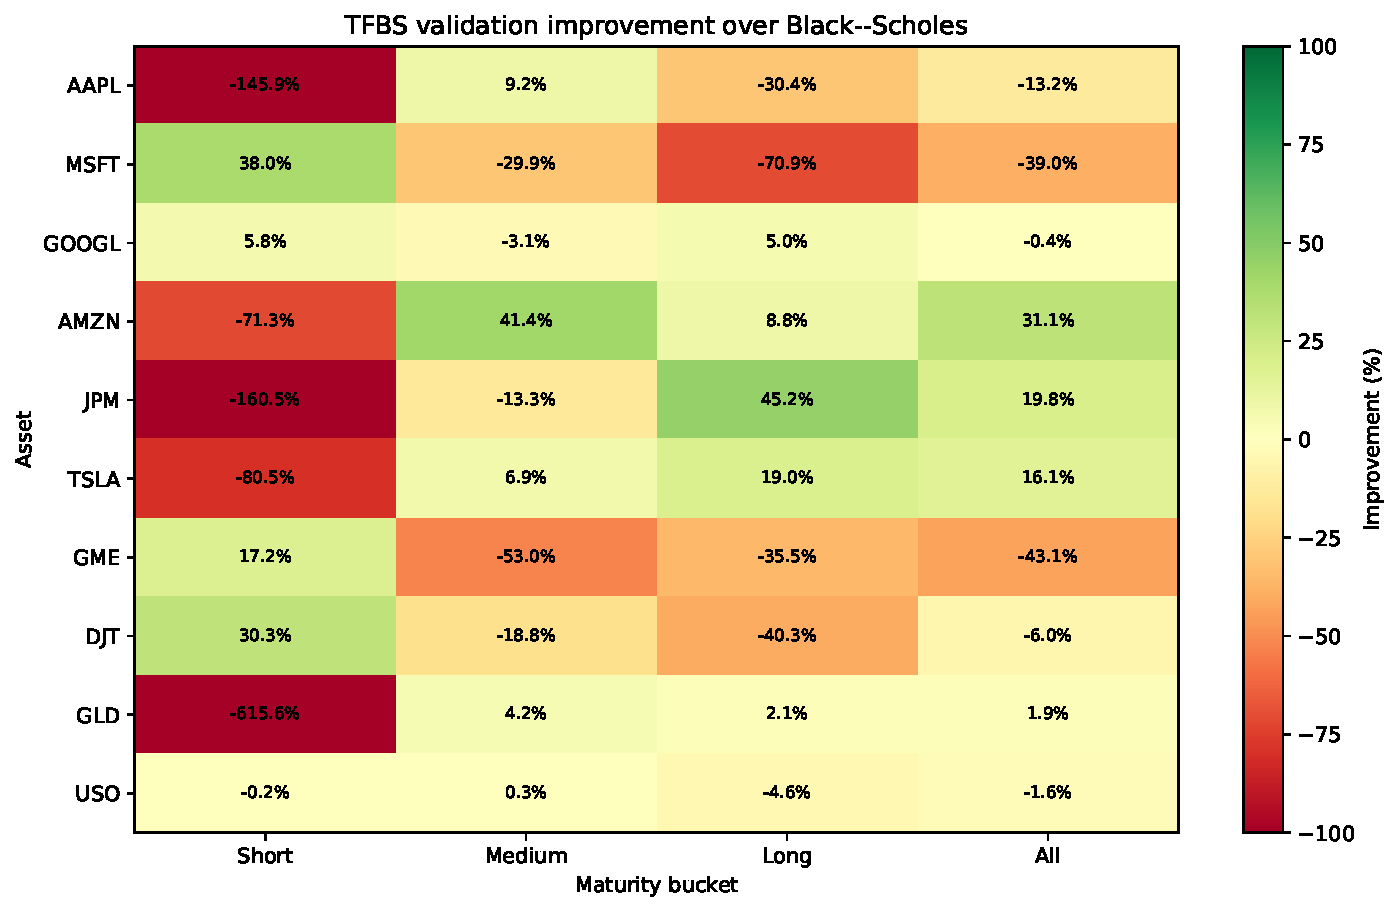
\includegraphics[width=0.92\textwidth]{fig7_1_cross_asset_improvement_heatmap.pdf}
\caption{Validation RMSE improvement of TFBS relative to Black--Scholes across assets and maturity buckets. The color scale is clipped at $\pm100\%$ for readability.}
\label{fig:cross_asset_improvement_heatmap}
\end{figure}

Table~\ref{tab:cross_asset_summary} summarizes validation RMSE and improvement for each asset and maturity bucket. For the short bucket, many assets have only one expiry, so short-maturity results should be interpreted with caution because they are based on a small sample and are sensitive to market microstructure noise. The main interpretation in this chapter therefore emphasizes the medium, long, and all-bucket results.

\begin{table}[htbp]
\centering
\scriptsize
\begin{tabular}{llrrrr}
\toprule
Asset & Bucket & $n_{\mathrm{exp}}$ & $RMSE^{BS}$ & $RMSE^{TFBS}$ & Improvement \\
\midrule
AAPL & Short  & 1 & 0.2667 & 0.6560 & $-145.9\%$ \\
AAPL & Medium & 5 & 0.6775 & 0.6150 & $9.2\%$ \\
AAPL & Long   & 3 & 0.7515 & 0.9803 & $-30.4\%$ \\
AAPL & All    & 9 & 0.6717 & 0.7604 & $-13.2\%$ \\
\midrule
MSFT & Short  & 1 & 0.4964 & 0.3078 & $38.0\%$ \\
MSFT & Medium & 5 & 0.4849 & 0.6298 & $-29.9\%$ \\
MSFT & Long   & 3 & 0.4740 & 0.8101 & $-70.9\%$ \\
MSFT & All    & 9 & 0.4826 & 0.6706 & $-39.0\%$ \\
\midrule
GOOGL & Short  & 1 & 1.3858 & 1.3053 & $5.8\%$ \\
GOOGL & Medium & 5 & 1.7936 & 1.8497 & $-3.1\%$ \\
GOOGL & Long   & 3 & 1.4600 & 1.3872 & $5.0\%$ \\
GOOGL & All    & 9 & 1.6466 & 1.6527 & $-0.4\%$ \\
\midrule
AMZN & Short  & 1 & 0.1251 & 0.2142 & $-71.3\%$ \\
AMZN & Medium & 5 & 0.5105 & 0.2991 & $41.4\%$ \\
AMZN & Long   & 3 & 0.3523 & 0.3213 & $8.8\%$ \\
AMZN & All    & 9 & 0.4334 & 0.2987 & $31.1\%$ \\
\midrule
JPM & Short  & 1 & 0.2227 & 0.5800 & $-160.5\%$ \\
JPM & Medium & 5 & 0.7195 & 0.8153 & $-13.3\%$ \\
JPM & Long   & 3 & 1.3800 & 0.7566 & $45.2\%$ \\
JPM & All    & 9 & 0.9633 & 0.7730 & $19.8\%$ \\
\midrule
TSLA & Short  & 1 & 0.1743 & 0.3145 & $-80.5\%$ \\
TSLA & Medium & 5 & 0.7447 & 0.6935 & $6.9\%$ \\
TSLA & Long   & 3 & 1.9223 & 1.5575 & $19.0\%$ \\
TSLA & All    & 9 & 1.2422 & 1.0425 & $16.1\%$ \\
\midrule
GME & Short  & 1 & 0.0661 & 0.0547 & $17.2\%$ \\
GME & Medium & 4 & 0.1256 & 0.1921 & $-53.0\%$ \\
GME & Long   & 3 & 0.1535 & 0.2080 & $-35.5\%$ \\
GME & All    & 8 & 0.1298 & 0.1857 & $-43.1\%$ \\
\midrule
DJT & Short  & 1 & 0.3182 & 0.2218 & $30.3\%$ \\
DJT & Medium & 5 & 0.2481 & 0.2948 & $-18.8\%$ \\
DJT & Long   & 2 & 0.1542 & 0.2163 & $-40.3\%$ \\
DJT & All    & 8 & 0.2490 & 0.2639 & $-6.0\%$ \\
\midrule
GLD & Short  & 1 & 0.1168 & 0.8360 & $-615.6\%$ \\
GLD & Medium & 5 & 1.0695 & 1.0242 & $4.2\%$ \\
GLD & Long   & 4 & 5.9478 & 5.8233 & $2.1\%$ \\
GLD & All    & 10 & 3.8372 & 3.7628 & $1.9\%$ \\
\midrule
USO & Short  & 1 & 2.7622 & 2.7664 & $-0.2\%$ \\
USO & Medium & 4 & 3.3815 & 3.3699 & $0.3\%$ \\
USO & Long   & 3 & 3.2305 & 3.3800 & $-4.6\%$ \\
USO & All    & 8 & 3.2534 & 3.3044 & $-1.6\%$ \\
\bottomrule
\end{tabular}
\caption{Cross-asset validation performance of BS and TFBS by maturity bucket.}
\label{tab:cross_asset_summary}
\end{table}

\section{Blue-Chip Equities}

Consider first the liquid blue-chip equity group, which includes AAPL, MSFT, GOOGL, AMZN, and JPM. Although these are large-cap equities with relatively high liquidity, the results are quite heterogeneous. Being a blue-chip stock does not by itself determine TFBS performance.

AMZN is the clearest positive case within the blue-chip group. In the medium bucket, TFBS reduces validation RMSE by about $41.4\%$ relative to Black--Scholes, and in the long bucket it produces an improvement of about $8.8\%$. The all-bucket improvement is about $31.1\%$. This suggests that the memory-tempering structure estimated by TFBS generalizes relatively well to validation strikes for the AMZN option surface.

By contrast, MSFT appears as a clear negative case. Although the short bucket shows positive improvement, it contains only one expiry and should not be interpreted strongly. In the medium bucket, improvement is $-29.9\%$, and in the long bucket it is $-70.9\%$. The all-bucket improvement is also negative at $-39.0\%$, meaning that TFBS performs worse than the Black--Scholes benchmark on validation strikes. This shows that the additional flexibility of TFBS does not necessarily translate into better generalization for all blue-chip option surfaces.

AAPL and GOOGL are closer to weak or mixed cases. AAPL shows an improvement of about $9.2\%$ in the medium bucket, but negative results in the long and all buckets. GOOGL shows weak positive improvement in the short and long buckets, but it is nearly neutral or weakly negative in the medium and all buckets. These assets therefore illustrate cases in which TFBS may improve performance for some maturities but does not provide a stable overall advantage.

JPM is a long-driven improvement case. In the medium bucket, TFBS performs worse than Black--Scholes with an improvement of $-13.3\%$. In the long bucket, however, TFBS improves validation RMSE by $45.2\%$, and the all-bucket improvement is about $19.8\%$. This indicates that the TFBS improvement for JPM occurs mainly in the long maturity region rather than in the medium maturity region.

Overall, TFBS validation performance varies substantially even within the blue-chip group. AMZN can be classified as a strong positive case, MSFT as a negative case, GOOGL as a near-neutral case, AAPL as a mixed case, and JPM as a long-driven positive case. This suggests that TFBS performance depends more on the maturity structure and memory-tempering signature of each asset's option surface than on whether the asset is a liquid blue-chip stock.

\section{High-Attention and Event-Driven Equities}

Next, consider the high-attention or event-driven equity group, which includes TSLA, GME, and DJT. These assets may be strongly affected by retail attention, event risk, speculative demand, and jump-like movements, making it difficult for a stable memory structure to emerge.

TSLA shows the most favorable result within this group. Although TFBS performs worse than Black--Scholes in the short bucket, it improves validation RMSE by about $6.9\%$ in the medium bucket and about $19.0\%$ in the long bucket. The all-bucket improvement is about $16.1\%$. This indicates that TFBS can produce lower validation error than Black--Scholes for TSLA in some maturity regions, especially the medium-to-long range. However, the improvement is smaller than that of AMZN, and because TSLA is a high-attention asset, the maturity-specific results should be interpreted cautiously.

GME and DJT, in contrast, illustrate event-driven instability. GME shows positive improvement in the short bucket, but TFBS performs worse in the medium bucket ($-53.0\%$), the long bucket ($-35.5\%$), and the all bucket ($-43.1\%$). DJT also shows positive improvement in the short bucket, but negative results in the medium and long buckets, and an all-bucket improvement of about $-6.0\%$.

These results suggest that TFBS performance can be unstable for high-attention or event-driven equities. Although TFBS improves some maturity buckets for TSLA, speculative demand, event risk, and liquidity imbalance may dominate option prices for GME and DJT, preventing the memory-tempering structure of TFBS from generalizing reliably to validation strikes.

\section{Commodity and Spot-Linked ETFs}

Finally, consider the commodity or spot-linked ETF group, which includes GLD and USO. These assets may be more strongly influenced by commodity cycles, macro factors, and futures market structure than by firm-specific earnings or news.

GLD shows very weak positive improvement in the medium and long buckets. The improvement is about $4.2\%$ in the medium bucket and about $2.1\%$ in the long bucket, with an all-bucket improvement of about $1.9\%$. The short bucket shows a large negative value, but this should not be interpreted strongly because the short bucket contains only one expiry and percentage measures can be unstable when RMSE values are small.

USO is essentially a neutral or weak negative case. It has a very small positive improvement of about $0.3\%$ in the medium bucket, but negative results in the long and all buckets. The all-bucket improvement is about $-1.6\%$.

The results for commodity-linked ETFs suggest that the additional explanatory power of TFBS may not appear in the same way as for equity options. For GLD and USO, the improvement is weak or mixed, suggesting that macro factors, commodity cycles, and futures market structure may play a more dominant role in shaping the option surface.

\section{Medium-Bucket Performance}

This thesis is particularly interested in whether TFBS improvement is more pronounced in the medium maturity region. Figure~\ref{fig:medium_improvement} shows the medium-bucket improvement for each asset. The figure indicates that medium-bucket results vary substantially by asset.

\begin{figure}[htbp]
\centering
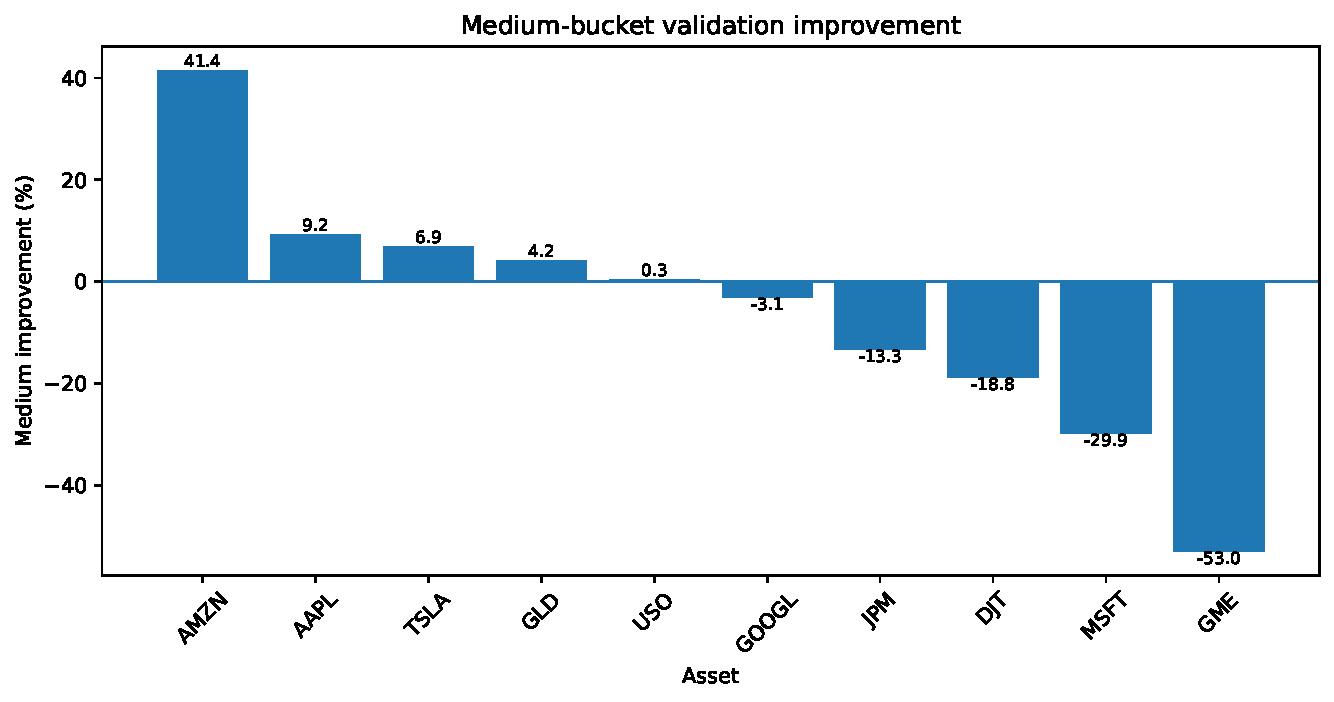
\includegraphics[width=0.85\textwidth]{fig7_2_medium_improvement.pdf}
\caption{Medium-bucket validation improvement of TFBS relative to Black--Scholes.}
\label{fig:medium_improvement}
\end{figure}

The strongest medium-bucket improvement is observed for AMZN. Its medium improvement is about $41.4\%$, making it the strongest positive medium-maturity case in the experiment. AAPL, TSLA, GLD, and USO also show positive medium-bucket improvement, but the magnitudes are relatively small. MSFT, GOOGL, JPM, GME, and DJT show negative medium-bucket results.

Thus, the experiment shows that a medium-maturity advantage for TFBS appears for some assets, but the effect is asset-specific. The medium maturity range alone does not automatically guarantee TFBS improvement.

\section{Validation RMSE Term Structures}

Figure~\ref{fig:selected_rmse_term_structures} shows validation RMSE term structures for four representative assets: AMZN, MSFT, TSLA, and GLD. AMZN represents a positive blue-chip case, MSFT a negative blue-chip case, TSLA a moderately positive high-attention case, and GLD a weakly positive or near-neutral commodity-linked ETF case.

\begin{figure}[htbp]
\centering
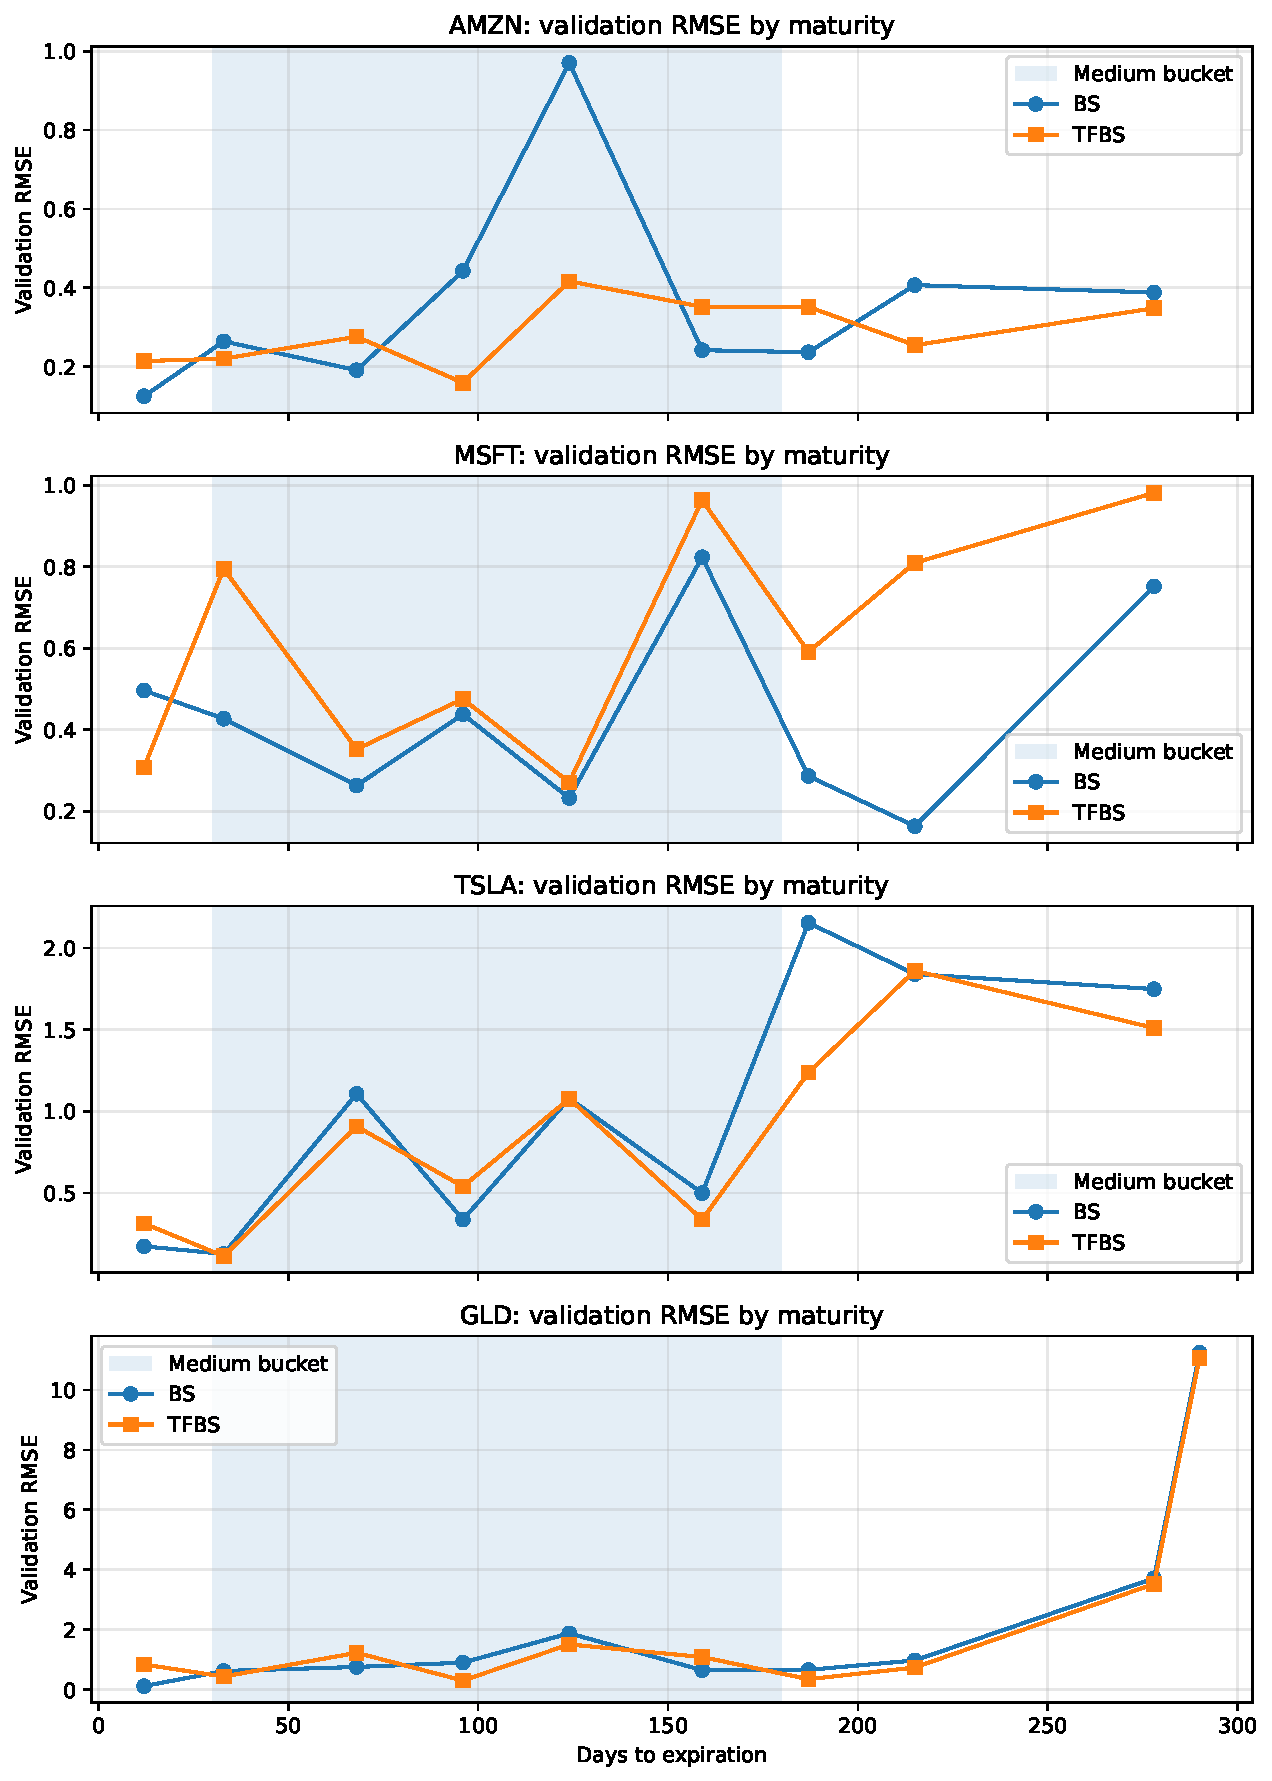
\includegraphics[width=0.9\textwidth]{fig7_3_selected_rmse_term_structures.pdf}
\caption{Validation RMSE term structures for selected representative assets. The shaded region denotes the medium-maturity bucket.}
\label{fig:selected_rmse_term_structures}
\end{figure}

For AMZN, TFBS RMSE is lower than Black--Scholes RMSE in the medium and long maturity regions. This suggests that AMZN's positive improvement is not merely a single-bucket artifact, but a pattern visible across the maturity term structure. In contrast, MSFT has higher TFBS RMSE in the medium and long maturity regions, consistent with its negative bucket-level results.

For TSLA, TFBS is less favorable at short maturities but shows some improvement in the medium and long maturity regions. This indicates that TFBS does not completely fail for high-attention assets, but the results may be less stable by maturity. For GLD, the difference between the two models' RMSE values is generally small, suggesting that the additional explanatory power of TFBS may be limited for commodity-linked ETFs.

\section{TFBS Parameter Signatures}

Validation performance alone does not reveal how TFBS explains the option surface. This section therefore examines the asset-level structure of the calibrated $\alpha$ and $\lambda$ values. Figure~\ref{fig:parameter_signatures} shows the calibrated fractional order $\widehat{\alpha}$ for each asset and the average tempering parameter $\widehat{\lambda}$ by maturity bucket.

\begin{figure}[htbp]
\centering
\begin{subfigure}{0.48\textwidth}
\centering
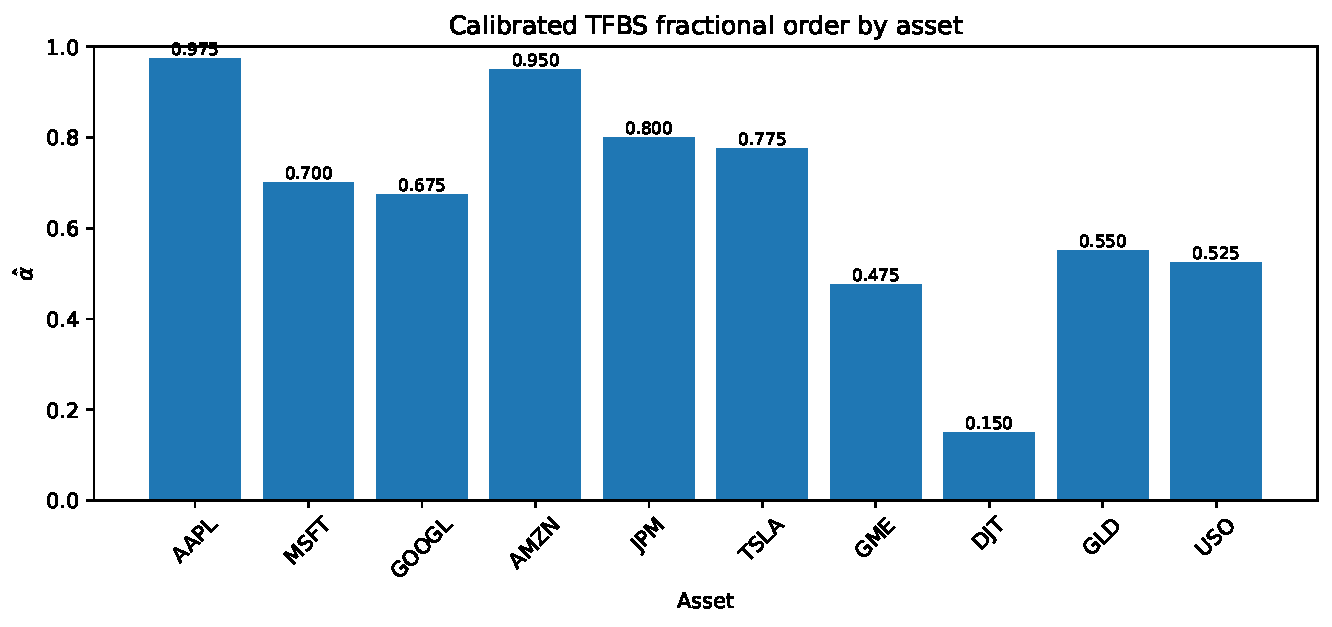
\includegraphics[width=\textwidth]{fig7_4a_alpha_by_asset.pdf}
\caption{Calibrated fractional order.}
\end{subfigure}
\hfill
\begin{subfigure}{0.48\textwidth}
\centering
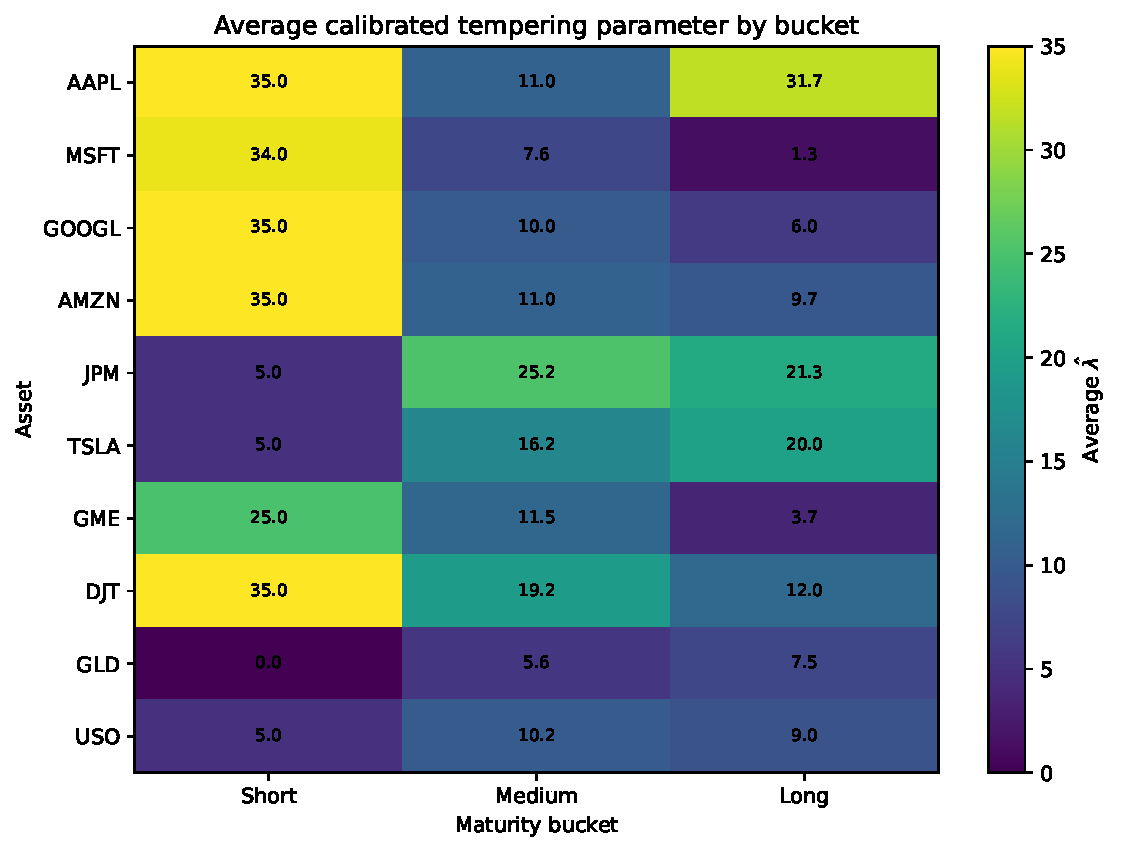
\includegraphics[width=\textwidth]{fig7_4b_lambda_bucket_heatmap.pdf}
\caption{Average tempering parameter by maturity bucket.}
\end{subfigure}
\caption{TFBS parameter signatures across assets.}
\label{fig:parameter_signatures}
\end{figure}

The calibrated $\widehat{\alpha}$ varies substantially across assets. AAPL and AMZN have values close to one, $0.975$ and $0.950$, respectively. This can be interpreted as meaning that TFBS uses a weak fractional correction close to the classical time derivative rather than a strong fractional-memory effect for these assets. By contrast, GME, GLD, and USO have lower $\widehat{\alpha}$ values, and DJT has a very low $\widehat{\alpha}$. However, a low $\alpha$ does not necessarily imply good validation performance. For example, GME has a low $\alpha$ but negative overall validation performance. Thus, $\alpha$ alone cannot explain TFBS performance.

The tempering parameter $\lambda$ also varies substantially across assets and maturity buckets. Some assets repeatedly select high $\lambda$ values. This suggests that TFBS may prefer rapidly decaying, strongly tempered memory rather than persistent long memory. However, if high $\lambda$ values are repeatedly selected, possible grid-boundary effects should be considered, and the parameter interpretation should be made cautiously.

AMZN is particularly notable because it is a strong positive case even though its $\alpha$ is close to one. This shows that TFBS improvement does not necessarily arise only from strong fractional memory; it can also arise from the combination of a weak fractional correction and a tempering structure. Conversely, GME and DJT may exhibit low $\alpha$ or high tempering parameters, but their validation improvement is not stable. Therefore, TFBS parameters should be interpreted jointly with validation performance as a memory-tempering signature rather than in isolation.

\section{Summary of Empirical Findings}

The cross-asset empirical results of this chapter can be summarized as follows.

First, the TFBS model does not universally improve upon the Black--Scholes benchmark for all assets and maturity buckets. Some assets show positive improvement, while others show weak, mixed, or negative results.

Second, it is not true that TFBS is always superior in the medium maturity bucket. AMZN is the strongest positive medium-bucket case, but MSFT, GME, DJT, and JPM show negative results in the medium bucket. Therefore, the medium-maturity advantage should be interpreted as an asset-specific phenomenon rather than a universal property.

Third, results are heterogeneous even within the blue-chip group. AMZN is a strong positive case, MSFT is a negative case, and GOOGL is near neutral. JPM is a long-driven case in which improvement occurs mainly in the long maturity bucket rather than the medium bucket. Thus, being a liquid blue-chip equity does not determine TFBS performance.

Fourth, the high-attention or event-driven equity group shows unstable results. TSLA exhibits moderate improvement in the medium and long buckets, whereas GME and DJT show negative validation performance. This suggests that when event risk, speculative demand, and liquidity conditions dominate the option surface, the memory-tempering structure of TFBS may not generalize reliably.

Fifth, the additional explanatory power of TFBS is weak for commodity-linked ETFs. GLD and USO are overall weak or near-neutral cases, suggesting that commodity cycles and macro factors may dominate their option surfaces.

Overall, the results support interpreting the TFBS model not as a universal pricing formula, but as a memory-diagnostic pricing model for assessing whether a finite-horizon memory structure is present in a particular option surface. The next chapter discusses candidate drivers that may explain asset-dependent differences in performance.


\chapter{Candidate Drivers of Asset-Dependent Performance}

\section{Overview}

The cross-asset empirical results in Chapter 7 show that the TFBS model does not uniformly improve upon the Black--Scholes benchmark for all assets and maturities. Some assets show lower validation RMSE in the medium or long maturity bucket, while others show weak or negative improvement. TFBS performance should therefore be interpreted as maturity-dependent and asset-specific rather than as universal model performance.

This chapter discusses candidate drivers that may explain these performance differences. The main candidate drivers are
\[
\begin{aligned}
&\text{(i) stable finite-horizon memory structure},\\
&\text{(ii) short-maturity noise and payoff nonlinearity},\\
&\text{(iii) option-surface smoothness and generalization},\\
&\text{(iv) high-attention and event-driven instability},\\
&\text{(v) commodity and macro-factor dominance}.
\end{aligned}
\]
These factors can operate simultaneously across assets and maturity buckets.

\section{Stable Finite-Horizon Memory Structure}

The most important condition for TFBS to perform well is the presence of a stable finite-horizon memory structure in the option surface. The memory kernel of TFBS is
\[
K_{\alpha,\lambda}(u)
=
e^{-\lambda u}u^{-\alpha}.
\]
Here $\alpha$ represents the shape of fractional memory, and $\lambda$ controls how quickly the memory effect decays with the time lag. Thus, TFBS does not simply assume that past information has a long-lasting influence. Instead, it can represent a structure in which the influence of past information gradually weakens within a finite horizon.

Assets with positive validation improvement in Chapter 7 can be interpreted as cases in which this finite-horizon memory structure generalizes to validation strikes. For example, AMZN shows the clearest positive improvement in the medium bucket. This suggests that the memory-tempering structure estimated from calibration strikes for AMZN can be applied relatively stably to validation strikes.

However, such a structure does not appear for every asset. Even within the same blue-chip group, AAPL, GOOGL, MSFT, and JPM display different results. Therefore, it is difficult to conclude that liquidity or blue-chip status alone determines TFBS performance. What matters is whether the option surface can stably reflect a TFBS-type memory-tempering structure across maturity and strike.

\section{Short-Maturity Noise and Payoff Nonlinearity}

In the short maturity bucket, TFBS performance is unstable for many assets. This may occur because short maturity options are more strongly affected by market microstructure noise and payoff nonlinearity than by model-implied memory structure.

First, as time to maturity becomes short, the kink in the call payoff $(S-K)^+$ has a stronger influence on option prices. Near the at-the-money region, gamma sensitivity can be high, so small changes in the underlying price or quotes can lead to large changes in option prices. This makes calibration of a smooth PDE-based pricing model difficult.

Second, short maturity options are sensitive to market microstructure effects such as bid--ask spreads, low trading volume, and stale lastPrice observations. The data source in this thesis is public option-chain data, and in some experiments the last transaction price is used as the market price proxy instead of the bid--ask midpoint. Since lastPrice reflects the price at the last execution time, it may differ from the current quote. This issue can strongly affect validation RMSE, especially for short maturity options.

Third, the short bucket often contains a small number of expiries. Although this study uses target DTE selection, the actual option chain may provide only a limited number of short-bucket expiries. As a result, the short-bucket improvement percentage can be driven by one or two expiries. For these reasons, this thesis uses short-bucket results as supporting evidence rather than as the main basis for conclusions, and interprets them together with medium- and long-bucket results.

\section{Option-Surface Smoothness and Generalization}

The TFBS model contains more parameters than the Black--Scholes model. It may therefore fit the calibration set better, but such improvement is meaningful only if it also holds in the validation set. This requires the option surface to be sufficiently smooth and stable, so that the structure in $(\alpha,\sigma,\lambda)$ estimated from calibration strikes generalizes to validation strikes.

From this perspective, differences in TFBS performance may be related to option-surface smoothness. For some assets, option prices vary relatively smoothly across strikes and maturities, and the memory-tempering structure captured by TFBS is also present at validation strikes. In such cases, TFBS may produce lower validation RMSE than the Black--Scholes benchmark. If the option surface moves irregularly at particular strikes or maturities, however, the additional TFBS parameters may fit the calibration set but fail to generalize to the validation set.

The blue-chip results in Chapter 7 illustrate this point. Within the same liquid blue-chip group, AMZN is a strong positive case in the medium bucket, while MSFT has negative performance in the medium and long buckets. GOOGL is close to neutral, and JPM shows improvement mainly in the long bucket rather than the medium bucket. This suggests that TFBS performance depends strongly on the smoothness and maturity structure of each asset's option surface, not merely on the asset-class label.

\section{High-Attention and Event-Driven Instability}

TFBS performance can be more unstable for high-attention or event-driven equities. Assets such as TSLA, GME, and DJT may be strongly affected by retail attention, speculative demand, event risk, and jump-like movements. These effects may appear in option prices as sudden price movements or sentiment shocks, rather than as a smooth memory kernel.

For TSLA, moderate improvement appears in the medium and long buckets, but negative performance appears in the short bucket. This suggests that TFBS can produce lower validation error than Black--Scholes in some maturity regions of the TSLA option surface, but the structure is not stable across all maturities.

GME and DJT show more unstable results. For these assets, event risk and speculative demand may dominate option prices. In such cases, the TFBS memory-tempering structure may not generalize reliably to validation strikes. In particular, when high values of $\lambda$ are estimated for high-attention assets, this may reflect the model attempting to capture rapidly decaying event-driven memory or attention effects rather than persistent long memory. The high-attention group therefore provides an important comparison group showing the limitations and parameter instability of TFBS.

\section{Commodity and Macro-Factor Dominance}

For commodity or spot-linked ETFs, different factors may dominate the option surface compared with equity options. GLD and USO are linked to gold and oil market factors, respectively. Their option prices may be more sensitive to commodity cycles, macro factors, dollar movements, inflation expectations, and futures market structure than to firm-specific earnings or news.

In Chapter 7, GLD and USO show weak or near-neutral TFBS improvement. This suggests that in commodity-linked ETF option surfaces, the component explained by a finite-horizon memory kernel may be limited. In particular, long maturity options may be strongly affected by macroeconomic uncertainty and commodity-specific risk, so a simple memory-tempering structure may not substantially improve validation performance.

This result indicates that TFBS may have some explanatory power for certain equity option surfaces, but its effect may be weaker for commodity-linked ETF option surfaces. It is therefore consistent with the asset-specific interpretation of this thesis.

\section{Summary of Candidate Drivers}

Table~\ref{tab:candidate_drivers} summarizes the candidate drivers discussed in this chapter. It links each driver to an expected empirical pattern and an interpretation.

\begin{table}[htbp]
\centering
\small
\begin{tabular}{p{0.22\textwidth}p{0.30\textwidth}p{0.34\textwidth}}
\toprule
Candidate driver & Expected empirical pattern & Interpretation \\
\midrule
Stable finite-horizon memory
&
Positive validation improvement in medium or long maturity; moderate and interpretable $\lambda$
&
TFBS captures a memory structure that generalizes from calibration strikes to validation strikes.
\\
\midrule
Short-maturity noise
&
Unstable or negative short-bucket improvement
&
Payoff kink, high gamma sensitivity, bid--ask noise, and stale price effects dominate short maturities.
\\
\midrule
Option-surface smoothness
&
Improvement differs even within the same asset class
&
Asset class label alone is insufficient; the smoothness and stability of each option surface matter.
\\
\midrule
Event-driven instability
&
High or unstable $\lambda$, mixed validation performance in high-attention assets
&
TFBS may capture short-lived event or attention effects rather than stable long memory.
\\
\midrule
Commodity and macro factors
&
Weak or near-neutral improvement for commodity-linked ETFs
&
Macro and commodity-specific risk may dominate the option surface.
\\
\bottomrule
\end{tabular}
\caption{Candidate drivers of asset-dependent TFBS performance.}
\label{tab:candidate_drivers}
\end{table}

Overall, the cross-asset differences should not be interpreted as evidence that TFBS is universally superior or inferior to Black--Scholes. Rather, they suggest that TFBS is useful when the option surface contains a stable finite-horizon memory structure that can be captured by $\alpha$ and $\lambda$. When option prices are dominated by short-maturity noise, event-driven jumps, or macro-commodity factors, the additional flexibility of TFBS may not translate into improved validation performance.

The central interpretation of this thesis is therefore that the TFBS model is not a universal pricing formula, but a diagnostic pricing model for checking whether an option surface contains memory-tempering structure. The next chapter summarizes robustness checks and model limitations, including grid sensitivity, price source, numerical resolution, maturity bucket definitions, and the calibration--validation split.

\chapter{Robustness Checks and Limitations}

\section{Overview}

Chapter 7 compared the validation performance of the TFBS model and the Black--Scholes benchmark across multiple underlying assets, and Chapter 8 discussed candidate drivers of the performance differences. This chapter summarizes robustness issues and limitations that should be considered when interpreting the empirical results.

TFBS performance depends on maturity bucket, asset class, option-surface structure, market price proxy, and parameter grid. Therefore, the empirical results should be interpreted as conditional on a particular data source, filtering rule, parameter grid, numerical resolution, and calibration--validation split.

The chapter discusses five main aspects:
\[
\begin{aligned}
&\text{(i) parameter grid sensitivity},\\
&\text{(ii) market price proxy and price-source limitation},\\
&\text{(iii) numerical resolution},\\
&\text{(iv) maturity bucket and validation split},\\
&\text{(v) model specification limitations}.
\end{aligned}
\]
The purpose of this discussion is to avoid overstating the empirical findings and to clarify the range within which the TFBS model should be interpreted.

\section{Grid Sensitivity and Parameter Boundary}

The TFBS model contains the fractional order $\alpha$, volatility parameter $\sigma$, and tempering parameter $\lambda$. Calibration results may therefore be affected by the range and resolution of the parameter grid. This thesis uses a coarse-to-fine grid strategy to reduce computational cost: a coarse grid first searches for a broad parameter region, and a local fine grid is then constructed around the coarse optimum for each maturity.

Finite grid search, however, has several limitations. First, the true optimum may lie between grid points. In that case, the estimated parameter is the closest grid point and contains discretization error. Second, if the optimal parameter is repeatedly selected near a grid boundary, the possibility that the true optimum lies outside the grid cannot be ruled out. In particular, if high values of $\lambda$ are repeatedly selected, one should consider both the interpretation that TFBS prefers strongly tempered memory and the possibility that the $\lambda$ grid may not be sufficiently wide.

Some assets in this study select high $\lambda$ values. This can be consistent with the interpretation that a rapidly decaying memory structure is more suitable than persistent long memory for those option surfaces. At the same time, high-$\lambda$ estimates may include parameter-boundary effects, so the numerical value of $\lambda$ should not be interpreted directly as the actual memory horizon of the market.

For this reason, the estimated $\alpha$ and $\lambda$ values in this thesis are interpreted not as structural physical parameters, but as model-implied memory signatures obtained through finite grid calibration. The important point is not the absolute value of a parameter, but the direction of the memory-tempering structure chosen by TFBS for each asset and maturity bucket, and whether it appears together with validation RMSE improvement.

\section{Market Price Proxy and Price-Source Limitation}

A major issue in applying an option pricing model to empirical data is the definition of the market price. Ideally, the bid--ask midpoint should be used. In public option-chain data, however, reliable bid and ask prices are not always available for every contract, and bid or ask prices may be reported as zero. In such cases, the last transaction price, or lastPrice, may have to be used as the market price proxy.

LastPrice has the advantage of being an actual executed price, but the last execution time may differ from the current observation time. Thus, lastPrice may be stale, and the problem can be especially severe for options with low trading volume or short maturities. Stale prices can substantially affect validation RMSE, so part of the observed model performance may reflect data noise rather than structural differences between pricing models.

The empirical results in this thesis should be interpreted with this public-data limitation in mind. Even if TFBS produces lower validation RMSE than Black--Scholes for a certain asset, it remains necessary to check whether the same result holds for bid--ask midpoint data. Conversely, if TFBS performs poorly for a certain asset, it may be difficult to separate whether this is due to the model structure itself or to stale lastPrice observations and liquidity issues.

Therefore, the empirical analysis in this thesis should be understood as a preliminary validation study based on public option data. Future work should use higher-quality quote-level data and jointly consider bid--ask midpoints, trade prices, quote timestamps, volume, and open interest.

\section{Numerical Resolution}

TFBS option prices are computed by a finite difference scheme rather than a closed-form formula. Therefore, numerical resolution, meaning the time grid size and space grid size, can affect pricing results. This thesis discretizes the time-to-maturity direction using $N$ time steps and the underlying-price direction using $M$ spatial intervals.

If the numerical resolution is too low, discretization error can be large. This is especially relevant for a fractional derivative because it contains a weighted history of past time increments; if time discretization is too coarse, the approximation of the memory term may be inaccurate. Conversely, choosing very large values of $M$ and $N$ greatly increases computational cost because the PDE solver must be run repeatedly for each parameter combination.

This thesis uses a moderate resolution for computational feasibility. It also distinguishes between the PDE resolution used in the coarse parameter search and the resolution used in final calibration. The initial scan uses a relatively low resolution, while final calibration uses a higher resolution. This design reflects the trade-off between computational cost and numerical accuracy.

The thesis does not provide a full convergence analysis. That is, it does not prove rigorously that the numerical solution converges to the theoretical TFBS solution as $M,N\to\infty$. The goal is instead to construct an empirical validation framework based on the TFBS PDE and compare model performance across assets and maturity buckets. Sensitivity to numerical resolution therefore remains a limitation and should be studied more systematically in future work.

\section{Maturity Bucket Sensitivity}

This thesis uses short, medium, and long maturity buckets to analyze maturity-dependent performance. The baseline classification is
\[
\text{Short}: T\le 30\ \text{days},
\]
\[
\text{Medium}: 30<T\le 180\ \text{days},
\]
and
\[
\text{Long}: T>180\ \text{days}.
\]
This classification is based on an intuitive segmentation commonly used in option-market analysis, but it is not absolute. For example, changing the upper bound of medium maturity from 180 days to 210 days could move some expiries from the medium bucket to the long bucket.

The arbitrariness of bucket boundaries should therefore be considered when interpreting medium-maturity advantage. If improvement for an asset is concentrated in an expiry close to 180 days, the medium-bucket result may change when the bucket definition is adjusted. If improvement appears stably across several medium-maturity expiries, it is less sensitive to the boundary.

In this thesis, maturity buckets are empirical groupings rather than theory-driven classifications. They are used to summarize model performance. It is therefore important to consider expiry-level results as well as pooled bucket-level RMSE. The RMSE term structures in Chapter 7 serve as a supporting tool for examining how bucket-level averages arise from individual maturities.

\section{Calibration--Validation Split Sensitivity}

Because the TFBS model contains more parameters than the Black--Scholes benchmark, comparing models only through in-sample calibration error is not appropriate. This thesis separates the strike set of each maturity into calibration and validation sets. The baseline split sorts strikes in increasing order and applies an alternating split.

This design has the advantage that both calibration and validation sets include in-the-money, near-the-money, and out-of-the-money strikes to some extent. However, validation results may depend on the split. If, for a given maturity, the validation set contains a stale price or abnormal quote, validation RMSE can be substantially distorted.

Moreover, the number of strikes used at each maturity is limited, so the validation set is also small. In the baseline design, a fixed number of near-the-money strikes is selected for each expiry, and some are used for calibration while the rest are used for validation. In this case, maturity-level validation RMSE can be affected by a small number of option contracts.

The validation results in this thesis should therefore be understood as split-specific. Stronger robustness could be obtained by using a reversed alternating split, repeated random splits, or a cross-validation-style strike split. This thesis presents a basic framework that separates in-sample fitting from out-of-sample validation, while leaving split sensitivity for future work.

\section{Model Specification Limitations}

The TFBS model in this thesis is a reduced-form PDE model that keeps the Black--Scholes spatial operator and replaces the time derivative with a tempered fractional derivative. This approach has the advantage of introducing a time-nonlocal memory effect while preserving a structure comparable with the Black--Scholes benchmark. However, it has several model-specification limitations.

First, the thesis does not provide a full no-arbitrage stochastic foundation. Introducing fractional Brownian motion or long-memory processes directly into the underlying asset dynamics can create complex issues related to no-arbitrage conditions. Rather than solving these issues, this study uses a reduced-form fractional PDE approach to test whether the option surface contains a finite-horizon memory structure.

Second, the PDE is based on a European-style call option pricing problem. However, equity options and ETF options traded in the U.S. market generally have American-style exercise features. Since this study focuses on call options and compares the Black--Scholes benchmark and the TFBS model under the same conditions, the main object of analysis is relative validation performance. Nevertheless, the impact of early exercise should be considered when interpreting absolute pricing accuracy.

Third, the interest rate and dividend yield are treated in a simplified way. Real option prices can be affected by the term structure of interest rates, discrete dividends, borrow costs, transaction costs, liquidity premia, and other market factors. This thesis does not aim to model all of these factors. Instead, it focuses on whether fractional time dynamics can improve validation pricing error relative to the Black--Scholes benchmark.

Fourth, the TFBS model does not directly model volatility smiles or jump risk. Its additional flexibility comes from fractional memory and tempering in the time direction. Therefore, for event-driven assets or assets with strong jump-like movements, the memory-tempering structure of TFBS may be insufficient to explain the option surface. This interpretation is consistent with the negative or unstable validation performance observed for high-attention assets such as GME and DJT.

\section{Interpretation of Empirical Findings}

Taking the robustness issues and limitations above into account, the empirical findings of this thesis should be interpreted as follows.

First, if TFBS shows positive validation improvement for a given asset, this does not imply that the model precisely describes the true pricing mechanism of that asset. It only means that the TFBS memory-tempering structure captures some features of the option surface better than the Black--Scholes benchmark.

Second, if TFBS shows negative validation improvement for a given asset, this does not imply that fractional modeling itself is meaningless. A negative result may mean that the asset's option surface is not well matched to the reduced-form memory structure of TFBS, or that data noise, split sensitivity, grid limitations, or event-driven effects are more important.

Third, the estimated $\alpha$ and $\lambda$ values are not physical memory parameters, but model-implied calibration parameters. They should be interpreted as diagnostic quantities describing the memory-tempering signature of each option surface within the TFBS model, rather than as direct measurements of market memory.

Fourth, the most important empirical result is heterogeneity rather than universal dominance. Some assets show positive improvement, some show weak or neutral results, and others show negative validation performance. This heterogeneity suggests that TFBS should be used as a diagnostic pricing model rather than a universal replacement for Black--Scholes.

\section{Summary}

This chapter summarized robustness issues and limitations relevant to the empirical results. Parameter grids, market price proxies, numerical resolution, maturity bucket definitions, and the calibration--validation split can all affect validation results. In addition, the TFBS model in this thesis is not a full no-arbitrage stochastic model, but a reduced-form PDE model that combines the Black--Scholes spatial operator with a tempered fractional time derivative.

Putting the results together, TFBS can be viewed as a memory-diagnostic pricing model for checking whether an option surface contains a finite-horizon memory structure. From this perspective, the cross-asset results in Chapter 7 and the candidate drivers in Chapter 8 show when TFBS may be useful and when its effect may be limited.

The next chapter summarizes the main findings of the thesis and discusses the mathematical meaning and empirical limitations of the TFBS model.

\chapter{Conclusion}

\section{Summary of the Thesis}

This thesis introduced the Tempered Fractional Black--Scholes (TFBS) model in order to extend the memory-free structure of the classical Black--Scholes model, and examined whether the model can reduce validation pricing error relative to the Black--Scholes benchmark on observed option data. The analysis focused not merely on whether the TFBS model fits calibration data better, but on out-of-sample pricing performance for validation strikes that are not used in calibration.

The Black--Scholes model is the most fundamental benchmark in option pricing theory. However, because it assumes constant volatility and uses a classical first-order derivative in the time direction, it does not directly include memory effects through which past market information may affect current option price dynamics non-locally. Fractional derivatives provide a natural way to address this limitation.

The simplest fractional extension is the FBS model, which replaces the time derivative of the Black--Scholes PDE with a Caputo fractional derivative. In the FBS model, however, the single fractional order $\alpha$ must describe both the shape of the memory kernel and the persistence of the memory effect. Preliminary experiments in this study also showed that the basic FBS model can produce unstable parameter estimates and unfavorable pricing performance, especially for short maturities. Based on these theoretical and preliminary empirical considerations, the thesis focused on the TFBS model, which uses an exponentially tempered Caputo derivative to separate memory shape from memory decay. The TFBS memory kernel has the form
\[
K_{\alpha,\lambda}(t)
=
e^{-\lambda t}t^{-\alpha},
\]
where $\alpha$ controls the shape of fractional memory and $\lambda$ controls the exponential decay of the memory effect.

Numerically, the TFBS PDE was discretized by combining an L1-type approximation for the tempered Caputo derivative with a finite difference method in the underlying-price direction. The discretized scheme reduces to a tridiagonal linear system at each time step, which is used to compute TFBS option prices for each strike and maturity. Each maturity's option chain was then divided into calibration and validation sets, and the TFBS model was compared with the Black--Scholes model using validation RMSE.

\section{Main Empirical Findings}

The empirical results show that the TFBS model does not uniformly improve upon the Black--Scholes benchmark for all assets and all maturity buckets. TFBS performance is not universal; it is maturity-dependent and asset-specific.

In the final unified experiment, the clearest positive case was AMZN. AMZN showed validation RMSE improvement of about $41.4\%$ in the medium bucket, about $8.8\%$ in the long bucket, and about $31.1\%$ in the all bucket. This suggests that the TFBS memory-tempering structure generalized relatively well from calibration strikes to validation strikes for the AMZN option surface.

MSFT, by contrast, appeared as a negative case. It showed negative improvement of about $-29.9\%$ in the medium bucket and $-70.9\%$ in the long bucket, and TFBS also performed worse than Black--Scholes in the all bucket. This shows that TFBS performance can differ substantially even within the same blue-chip group.

AAPL and GOOGL are closer to weak or mixed cases. AAPL showed weak positive improvement in the medium bucket but negative results in the long and all buckets. GOOGL showed validation RMSE close to that of Black--Scholes overall. JPM can be interpreted as a long-driven case, with negative performance in the medium bucket but positive improvement in the long bucket.

High-attention or event-driven equities showed more unstable results. TSLA displayed moderate improvement in the medium and long buckets but negative performance in the short bucket. GME and DJT showed negative validation performance in the medium and long buckets. This suggests that when event risk, speculative demand, and liquidity conditions dominate the option surface, the memory-tempering structure of TFBS may not generalize reliably to validation strikes.

For commodity or spot-linked ETFs such as GLD and USO, the additional explanatory power of TFBS was very weak. GLD showed weak positive improvement in the medium and long buckets but was nearly neutral overall, while USO was weakly negative in the all bucket. This suggests that macro factors, commodity cycles, and futures market structure may play a more important role than a memory kernel in commodity-linked ETF options.

Therefore, the empirical results show that TFBS improvement is conditional on the asset and maturity bucket rather than universal.

\section{Interpretation of the Results}

The results support interpreting the TFBS model as a memory-diagnostic pricing model that tests whether an option surface contains finite-horizon memory structure, rather than as a universal pricing formula.

The TFBS model has two memory-related parameters. The fractional order $\alpha$ determines the power-law shape of the memory kernel, and the tempering parameter $\lambda$ controls how quickly the memory effect decays with the time lag. However, the empirical results show that model performance cannot be explained by $\alpha$ or $\lambda$ alone. In some assets, positive validation improvement appears even when $\alpha$ is close to one and the fractional correction is weak. In other assets, validation performance is poor even when a low $\alpha$ or high $\lambda$ is selected.

Therefore, $\alpha$ and $\lambda$ should be interpreted not as physical parameters that directly measure actual market memory, but as model-implied memory signatures calibrated within the TFBS model to describe the option surface. What matters is not simply the magnitude of a parameter, but whether the parameter structure appears together with stable validation pricing performance.

The medium maturity results also require caution. The thesis started from the idea that the TFBS memory-tempering structure may appear more clearly in medium maturity options. Indeed, AMZN and TSLA show positive improvement in the medium bucket. However, MSFT, GME, DJT, and JPM show negative medium-bucket results. Thus, the medium maturity range does not automatically guarantee TFBS improvement. A more accurate conclusion is that a medium-maturity advantage can appear for some option surfaces, but it is asset-specific.

\section{Mathematical and Methodological Contributions}

The first contribution of this thesis is to organize Black--Scholes, FBS, and TFBS within a unified fractional PDE framework. In the time-to-maturity variable, the classical Black--Scholes PDE has the form
\[
\frac{\partial C}{\partial \tau}
=
\mathcal{L}_{BS}C.
\]
The FBS model replaces the classical derivative on the left-hand side with a Caputo fractional derivative, and the TFBS model further extends it to a tempered Caputo derivative. In particular, when $\lambda=0$, TFBS reduces to FBS, so TFBS is a natural extension that contains the untempered memory structure of FBS.

The second contribution is the construction of a numerical pricing scheme for the TFBS PDE. By discretizing the tempered Caputo derivative with an L1-type scheme and the Black--Scholes spatial operator with a finite difference method, the TFBS pricing problem is reduced to repeated solutions of a tridiagonal linear system. This provides a computational framework for applying the TFBS model to observed option chains even though it has no closed-form solution.

The third contribution is the use of a calibration--validation split to evaluate out-of-sample pricing performance. Because TFBS contains more parameters than Black--Scholes, comparing only calibration errors would not rule out in-sample overfitting. By dividing strikes at each maturity into calibration and validation sets and comparing validation RMSE, the thesis evaluates whether the additional flexibility of TFBS translates into actual validation performance.

Finally, the thesis shows through a cross-asset validation framework that TFBS performance is maturity-dependent and asset-specific. This supports interpreting TFBS not as a model justified by a single positive asset result, but as a diagnostic model that must be evaluated conditionally across different option surfaces.

\section{Limitations}

This thesis has several limitations. First, the empirical analysis is based on public option-chain data. In public data, the bid--ask midpoint is not always available in a reliable form, and some experiments use the last transaction price as the market price proxy. LastPrice may be stale, especially for short maturity options and contracts with low trading activity, and it may distort validation RMSE.

Second, the PDE framework in this thesis is based on a European-style call option pricing problem. Equity options and ETF options traded in the U.S. market generally have American-style exercise features. Although the thesis compares the Black--Scholes benchmark and the TFBS model under the same assumptions and focuses on relative validation performance, the early-exercise feature should be considered when interpreting absolute pricing accuracy.

Third, the interest rate and dividend yield are treated in a simplified way. Real option prices can be affected by the term structure of interest rates, discrete dividends, borrow costs, liquidity premia, transaction costs, and other market factors. This thesis does not aim to model all of these elements, but focuses on the additional explanatory power of fractional time dynamics from the perspective of validation RMSE.

Fourth, parameter calibration is based on finite grid search. The estimated values of $\alpha$, $\sigma$, and $\lambda$ may therefore depend on grid range and grid resolution. In particular, if high $\lambda$ values or values near the grid boundary are repeatedly selected, both a strongly tempered-memory interpretation and possible grid-boundary effects should be considered.

Fifth, the thesis does not provide a full no-arbitrage stochastic foundation. Introducing fractional Brownian motion or long-memory processes directly into the underlying dynamics can raise complex no-arbitrage issues \cite{Cheridito2003}. This thesis instead uses a reduced-form fractional PDE approach that keeps the Black--Scholes spatial operator and replaces the time derivative with a tempered fractional derivative.

\section{Future Work}

A natural extension of this study is to use higher-quality option data for robustness analysis. In particular, jointly considering bid--ask midpoints, quote timestamps, trade prices, volume, and open interest would allow stale prices and liquidity noise to be controlled more systematically.

Second, price-source robustness should be examined more clearly. The main results in this thesis often rely on lastPrice because of public-data limitations. Future work can compare midpoint-based prices and lastPrice-based prices to analyze how sensitive TFBS validation improvement is to the market price proxy.

Third, robustness to maturity bucket definitions should be studied. This thesis defines the short, medium, and long buckets as $T\le30$ days, $30<T\le180$ days, and $T>180$ days. If the boundary of the medium bucket is changed from 180 days to 210 days, for example, some expiry assignments may change. Future research can examine whether TFBS improvement is maintained across multiple maturity bucket definitions.

Fourth, a more rigorous convergence and stability analysis of the numerical scheme is needed. This thesis uses an L1 scheme and finite difference method to compute the TFBS PDE numerically, but it does not provide a full theoretical convergence proof. Future work can analyze stability conditions, consistency, and convergence rates for the tempered fractional PDE more rigorously.

Fifth, the TFBS model can be combined with other option pricing features. Stochastic volatility is treated systematically in the Heston model \cite{Heston1993}; fractional diffusion approaches have been studied for markets with jumps \cite{CarteaDelCastilloNegrete2007}; and rough volatility provides a separate non-Markovian volatility framework \cite{GatheralJaissonRosenbaum2018}. For event-driven assets or high-attention stocks, jump-like movements and speculative demand may dominate the option surface. In such cases, a pure memory-tempering structure may be insufficient, so hybrid models combining fractional time dynamics with jump or stochastic-volatility components may be considered.


\appendix

\chapter{Auxiliary Results in Fractional Calculus}

\section{Cauchy Formula for Repeated Integration}

This section proves Cauchy's formula for repeated integer-order integration. Let $f$ be integrable on $[0,T]$. For $n\in\mathbb{N}$, we show that
\[
(I^n f)(t)
=
\frac{1}{(n-1)!}
\int_0^t
(t-s)^{n-1}f(s)\,ds.
\]

For $n=1$,
\[
(I^1 f)(t)
=
\int_0^t f(s)\,ds,
\]
so the formula holds. Suppose that for some $n\ge1$,
\[
(I^n f)(t)
=
\frac{1}{\Gamma(n)}
\int_0^t
(t-s)^{n-1}f(s)\,ds.
\]
Then
\[
(I^{n+1}f)(t)
=
\int_0^t (I^n f)(u)\,du.
\]
Using the induction hypothesis and Fubini's theorem,
\[
\begin{aligned}
(I^{n+1}f)(t)
&=
\frac{1}{\Gamma(n)}
\int_0^t
\int_0^u
(u-s)^{n-1}f(s)\,ds\,du  \\
&=
\frac{1}{\Gamma(n)}
\int_0^t
f(s)
\left(
\int_s^t
(u-s)^{n-1}\,du
\right)ds  \\
&=
\frac{1}{n\Gamma(n)}
\int_0^t
(t-s)^n f(s)\,ds  \\
&=
\frac{1}{\Gamma(n+1)}
\int_0^t
(t-s)^n f(s)\,ds.
\end{aligned}
\]
Thus, by induction, Cauchy's formula holds for all $n\in\mathbb{N}$.

\section{Semigroup Property of Riemann--Liouville Fractional Integrals}

The Riemann--Liouville fractional integral satisfies a semigroup property under suitable conditions. For $\alpha,\beta>0$,
\[
I^\alpha I^\beta f
=
I^{\alpha+\beta}f.
\]
To verify this, use the definition:
\[
(I^\alpha I^\beta f)(t)
=
\frac{1}{\Gamma(\alpha)\Gamma(\beta)}
\int_0^t
(t-u)^{\alpha-1}
\left[
\int_0^u
(u-s)^{\beta-1}f(s)\,ds
\right]du.
\]
Applying Fubini's theorem gives
\[
(I^\alpha I^\beta f)(t)
=
\frac{1}{\Gamma(\alpha)\Gamma(\beta)}
\int_0^t
f(s)
\left[
\int_s^t
(t-u)^{\alpha-1}
(u-s)^{\beta-1}
\,du
\right]ds.
\]
In the inner integral, substitute $u=s+(t-s)y$. Then
\[
\int_s^t
(t-u)^{\alpha-1}
(u-s)^{\beta-1}
\,du
=
(t-s)^{\alpha+\beta-1}
\int_0^1
(1-y)^{\alpha-1}y^{\beta-1}\,dy.
\]
Using the beta-function identity
\[
B(\beta,\alpha)
=
\int_0^1
y^{\beta-1}(1-y)^{\alpha-1}\,dy
=
\frac{\Gamma(\alpha)\Gamma(\beta)}
{\Gamma(\alpha+\beta)},
\]
we obtain
\[
(I^\alpha I^\beta f)(t)
=
\frac{1}{\Gamma(\alpha+\beta)}
\int_0^t
(t-s)^{\alpha+\beta-1}f(s)\,ds
=
(I^{\alpha+\beta}f)(t).
\]

\section{Positivity and Monotonicity of the Tempered Memory Kernel}

The tempered memory kernel used in the TFBS model is
\[
K_{\alpha,\lambda}(u)
=
e^{-\lambda u}u^{-\alpha},
\qquad u>0,
\]
where $0<\alpha<1$ and $\lambda\ge0$.

Since $e^{-\lambda u}>0$ and $u^{-\alpha}>0$,
\[
K_{\alpha,\lambda}(u)>0.
\]
Also,
\[
\log K_{\alpha,\lambda}(u)
=
-\lambda u-\alpha\log u,
\]
and therefore
\[
\frac{d}{du}\log K_{\alpha,\lambda}(u)
=
-\lambda-\frac{\alpha}{u}<0.
\]
Thus, $K_{\alpha,\lambda}(u)$ is strictly decreasing for $u>0$. In particular, as $\lambda$ increases, exponential damping becomes stronger and the influence of the distant past decays more rapidly.

\section{Positivity of the Discrete L1 Weights}

The fractional weights used in the L1 scheme are defined by
\[
w_k
=
(k+1)^{1-\alpha}-k^{1-\alpha},
\qquad k=0,1,2,\dots,
\]
where $0<\alpha<1$.

Consider the function
\[
\phi(x)=x^{1-\alpha}.
\]
Since $0<1-\alpha<1$, the function $\phi$ is increasing and concave on $x>0$. Therefore, the forward difference
\[
w_k
=
\phi(k+1)-\phi(k)
\]
is positive, so
\[
w_k>0.
\]
Because $\phi$ is concave, the forward difference is decreasing. Hence
\[
w_{k+1}\le w_k.
\]

The tempered L1 weight is defined by
\[
\widetilde w_k
=
e^{-\lambda k\Delta t}w_k.
\]
Since $\lambda\ge0$, the exponential factor is also positive. Therefore,
\[
\widetilde w_k>0.
\]
Moreover, $e^{-\lambda k\Delta t}$ decreases in $k$, so tempering makes the past weights decay more rapidly.

\section{Limiting Case: Recovery of the Black--Scholes PDE}
\label{app:bs_limit}

This section verifies that the TFBS PDE recovers the classical Black--Scholes PDE in an appropriate parameter limit. The tempered Caputo derivative used in the TFBS model is defined by
\[
({}^C D_\tau^{\alpha,\lambda} f)(\tau)
=
\frac{1}{\Gamma(1-\alpha)}
\int_0^\tau
e^{-\lambda(\tau-s)}
(\tau-s)^{-\alpha}
f'(s)\,ds,
\qquad 0<\alpha<1,
\quad \lambda\ge0.
\]
If $\lambda=0$, the exponential tempering factor disappears and
\[
({}^C D_\tau^{\alpha,0} f)(\tau)
=
\frac{1}{\Gamma(1-\alpha)}
\int_0^\tau
(\tau-s)^{-\alpha}
f'(s)\,ds
=
({}^C D_\tau^\alpha f)(\tau).
\]
Thus, the TFBS operator reduces to the ordinary Caputo fractional derivative when $\lambda=0$.

Now consider the limit $\alpha \uparrow 1$. Let $\beta=1-\alpha$, so $\beta\downarrow0$. Then
\[
({}^C D_\tau^\alpha f)(\tau)
=
(I^{1-\alpha}f')(\tau)
=
(I^\beta f')(\tau),
\]
where
\[
(I^\beta g)(\tau)
=
\frac{1}{\Gamma(\beta)}
\int_0^\tau
(\tau-s)^{\beta-1}g(s)\,ds.
\]
For sufficiently smooth $f$, the Riemann--Liouville fractional integral converges to the identity operator as $\beta\downarrow0$. Hence
\[
\lim_{\alpha\uparrow1}
({}^C D_\tau^\alpha f)(\tau)
=
\lim_{\beta\downarrow0}
(I^\beta f')(\tau)
=
f'(\tau).
\]
Therefore,
\[
\boxed{
\lim_{\alpha\uparrow1}
({}^C D_\tau^{\alpha,0} f)(\tau)
=
\frac{df}{d\tau}(\tau)
}
\]
holds.

The same fact can also be checked through the Laplace transform. Let $F(z)=\mathcal{L}\{f\}(z)$. Then
\[
\mathcal{L}\{({}^C D_\tau^\alpha f)(\tau)\}(z)
=
z^\alpha F(z)-z^{\alpha-1}f(0).
\]
As $\alpha\uparrow1$,
\[
z^\alpha F(z)-z^{\alpha-1}f(0)
\longrightarrow
zF(z)-f(0)
=
\mathcal{L}\{f'(\tau)\}(z).
\]
Thus,
\[
{}^C D_\tau^\alpha f
\longrightarrow
\frac{df}{d\tau}
\qquad
\text{as } \alpha\uparrow1.
\]

Applying this result to the TFBS PDE,
\[
{}^C D_\tau^{\alpha,\lambda} C(S,\tau)
=
\mathcal{L}_{BS}C(S,\tau),
\]
where
\[
\mathcal{L}_{BS}C
=
\frac{1}{2}\sigma^2S^2C_{SS}
+
(r-q)SC_S
-
rC,
\]
the left-hand side converges to the classical first-order time derivative when $\lambda=0$ and $\alpha\uparrow1$. Therefore,
\[
\lim_{\alpha\uparrow1}
{}^C D_\tau^{\alpha,0} C(S,\tau)
=
\frac{\partial C}{\partial \tau}(S,\tau).
\]

The limiting equation is therefore
\[
\frac{\partial C}{\partial \tau}(S,\tau)
=
\mathcal{L}_{BS}C(S,\tau),
\]
that is,
\[
\frac{\partial C}{\partial \tau}
=
\frac{1}{2}\sigma^2S^2C_{SS}
+
(r-q)SC_S
-
rC.
\]
This is the classical Black--Scholes PDE in the time-to-maturity variable $\tau$.

The TFBS model in this thesis also uses the same call-option payoff
\[
C(S,0)=(S-K)^+
\]
and boundary conditions
\[
C(0,\tau)=0,
\qquad
C(S_{\max},\tau)
\approx
S_{\max}e^{-q\tau}-Ke^{-r\tau}
\]
as the Black--Scholes benchmark. Thus, in the limiting sense $\lambda=0$ and $\alpha\uparrow1$, the TFBS pricing problem recovers the classical Black--Scholes pricing problem.

\chapter{Numerical Scheme Details}

\section{Finite Difference Coefficients}

The spatial operator in the TFBS PDE is
\[
\mathcal{L}_{BS}C
=
\frac{1}{2}\sigma^2S^2C_{SS}
+
(r-q)SC_S
-
rC.
\]
Let the spatial grid be
\[
S_j=j\Delta S,
\qquad j=0,1,\dots,M,
\]
and use central difference approximations at interior points $j=1,\dots,M-1$:
\[
C_S(S_j,\tau_n)
\approx
\frac{C_{j+1}^n-C_{j-1}^n}{2\Delta S},
\]
\[
C_{SS}(S_j,\tau_n)
\approx
\frac{C_{j+1}^n-2C_j^n+C_{j-1}^n}{(\Delta S)^2}.
\]
Substituting these into $\mathcal{L}_{BS}$ yields
\[
(\mathcal{L}_hC^n)_j
=
A_jC_{j-1}^n
+
B_jC_j^n
+
D_jC_{j+1}^n,
\]
where
\[
A_j
=
\frac{1}{2}\sigma^2\frac{S_j^2}{(\Delta S)^2}
-
\frac{1}{2}(r-q)\frac{S_j}{\Delta S},
\]
\[
B_j
=
-\sigma^2\frac{S_j^2}{(\Delta S)^2}
-
r,
\]
and
\[
D_j
=
\frac{1}{2}\sigma^2\frac{S_j^2}{(\Delta S)^2}
+
\frac{1}{2}(r-q)\frac{S_j}{\Delta S}.
\]

\section{Fully Discrete Matrix Form}

Combining the L1 approximation with the implicit finite difference scheme gives, on the interior grid,
\[
a_0
\left[
C_j^{n+1}-C_j^n
+
\sum_{k=1}^{n}
\widetilde w_k
\left(
C_j^{n+1-k}-C_j^{n-k}
\right)
\right]
=
(\mathcal{L}_hC^{n+1})_j.
\]
Rearranging,
\[
a_0C_j^{n+1}
-
(\mathcal{L}_hC^{n+1})_j
=
a_0C_j^n
-
a_0
\sum_{k=1}^{n}
\widetilde w_k
\left(
C_j^{n+1-k}-C_j^{n-k}
\right).
\]

Let
\[
C_{\mathrm{int}}^n
=
(C_1^n,\dots,C_{M-1}^n)^\top.
\]
Then the fully discrete scheme can be written as
\[
(a_0I-L_h)C_{\mathrm{int}}^{n+1}
=
a_0C_{\mathrm{int}}^n
-
a_0H_{\mathrm{int}}^n
+
b_{\mathrm{bdry}}^{n+1},
\]
where
\[
H_{\mathrm{int}}^n
=
\sum_{k=1}^{n}
\widetilde w_k
\left(
C_{\mathrm{int}}^{n+1-k}
-
C_{\mathrm{int}}^{n-k}
\right)
\]
is the fractional history term.

\section{Tridiagonal Matrix Structure}

The matrix
\[
A_h=a_0I-L_h
\]
is tridiagonal. For each interior index, the diagonal and off-diagonal entries are
\[
(A_h)_{j,j}
=
a_0-B_j,
\]
\[
(A_h)_{j,j-1}
=
-A_j,
\]
and
\[
(A_h)_{j,j+1}
=
-D_j.
\]
Therefore, the linear system to be solved at each time step is
\[
A_hC_{\mathrm{int}}^{n+1}
=
R^n,
\]
where $R^n$ is the right-hand side containing option values from previous time levels and the boundary correction.

\section{Boundary Correction}

The call option boundary conditions are
\[
C(0,\tau)=0
\]
and
\[
C(S_{\max},\tau)
\approx
S_{\max}e^{-q\tau}
-
Ke^{-r\tau}.
\]
The equation for $j=1$ contains $C_0^{n+1}$, but $C_0^{n+1}=0$, so the left-boundary correction disappears. In contrast, the equation for $j=M-1$ contains $C_M^{n+1}$. Therefore, the known boundary value
\[
C_M^{n+1}
=
S_{\max}e^{-q\tau_{n+1}}
-
Ke^{-r\tau_{n+1}}
\]
is reflected on the right-hand side.

\section{Interpolation at the Current Underlying Price}

The finite difference scheme computes option values at grid points $S_j$. The actual current underlying price $S_0$ need not coincide with a grid point, so the final time-level price curve
\[
\{(S_j,C_j^N)\}_{j=0}^{M}
\]
is used to interpolate the option price at $S_0$. This thesis uses linear interpolation. If $S_j\le S_0\le S_{j+1}$, then
\[
C(S_0,T)
\approx
C_j^N
+
\frac{S_0-S_j}{S_{j+1}-S_j}
\left(
C_{j+1}^N-C_j^N
\right).
\]

\chapter{Reproducibility Details}
\label{app:reproducibility}

This appendix records the data snapshot, filtering rules, calibration grids, and numerical settings used in the final empirical run. The purpose of this appendix is not to reinterpret the empirical results, but to make the numerical experiment in Chapters 6 and 7 reproducible from the same code and data collection protocol.

The final run was produced from \texttt{TFBSv2.ipynb}, using the cell labelled \texttt{Fresh final run for Chapter 7}. The notebook output directory was \texttt{/content/tfbs\_final\_run}. Tables and figures were saved in the corresponding subdirectories. The market data snapshot used for this thesis was collected on 2026-06-14. Because the option chains are downloaded from a live public data source, re-running the notebook on a later date may lead to different option chains, underlying prices, strikes, and validation errors.

\section{Data Snapshot}

Table~\ref{tab:repro_asset_snapshot} summarizes the final asset universe and the basic data counts used in the unified run. The underlying price $S_0$ is the last close returned by the yfinance historical-price query at the time of collection. The column \textit{All} is the number of selected call-option contracts after filtering, and \textit{Cal.} and \textit{Val.} are the numbers of contracts assigned to the calibration and validation sets, respectively. The final column reports the asset-level calibrated fractional order $\widehat{\alpha}$ used for all maturities of the same asset.

\begin{table}[htbp]
\centering
\scriptsize
\begin{tabular}{llrrrrrr}
\toprule
Asset & Group & $S_0$ & Exp. & All & Cal. & Val. & $\widehat{\alpha}$ \\
\midrule
AAPL & Blue-chip & 291.13 & 9 & 72 & 36 & 36 & 0.975 \\
MSFT & Blue-chip & 390.74 & 9 & 72 & 36 & 36 & 0.700 \\
GOOGL & Blue-chip & 359.68 & 9 & 72 & 36 & 36 & 0.675 \\
AMZN & Blue-chip & 238.55 & 9 & 72 & 36 & 36 & 0.950 \\
JPM & Blue-chip & 320.72 & 9 & 72 & 36 & 36 & 0.800 \\
TSLA & High-att. & 406.43 & 9 & 72 & 36 & 36 & 0.775 \\
GME & High-att. & 21.77 & 8 & 61 & 31 & 30 & 0.475 \\
DJT & High-att. & 7.80 & 8 & 42 & 24 & 18 & 0.150 \\
GLD & ETF & 386.54 & 10 & 80 & 40 & 40 & 0.550 \\
USO & ETF & 125.43 & 8 & 64 & 32 & 32 & 0.525 \\
\bottomrule
\end{tabular}
\caption{Final data snapshot and asset-level fractional order in the unified run.}
\label{tab:repro_asset_snapshot}
\end{table}

\section{Market Data and Filtering Rules}

The empirical analysis uses call options from the selected asset universe. The option data are obtained from the public \texttt{yfinance} option-chain interface, and the underlying price is obtained from the corresponding historical price query. The following settings define the data collection and filtering protocol.

{\small
\begin{longtable}{p{0.28\textwidth}p{0.62\textwidth}}
\caption{Market data and filtering rules used in the final run.}
\label{tab:repro_market_rules}\\
\toprule
Item & Final setting \\
\midrule
Data interface & \texttt{yfinance.Ticker} for both underlying price history and option chains. \\
Underlying price & Last close from \texttt{history(period="1y", auto\_adjust=False)}. \\
Option type & Call options only. \\
DTE computation & Expiry date minus the UTC-normalized collection date. \\
Target DTEs & 14, 30, 60, 90, 120, 150, 180, 210, 270, and 360 days. For each target DTE, the nearest available expiry is selected; duplicate expiries are removed. \\
DTE range & Minimum DTE 0 days and maximum DTE 365 days. \\
Moneyness filter & $0.70 \leq K/S_0 \leq 1.30$. \\
Contracts per expiry & At most 8 strikes per expiry, selected by smallest $|K/S_0-1|$ and then sorted by strike. \\
Market price proxy & \texttt{lastPrice}. In the final run, all selected contracts have price type \texttt{last}. \\
Spread filter & No maximum spread filter; \texttt{max\_spread\_pct=None}. \\
Volume and open interest filters & No minimum volume or open-interest filter. \\
Maturity buckets & Short: $T\leq 30$ days; Medium: $30<T\leq 180$ days; Long: $T>180$ days. \\
\bottomrule
\end{longtable}
}

\section{Selected Expiries}

Table~\ref{tab:repro_selected_expiries} reports the exact expiries used for each asset in the final run. These are the expiries that survived the DTE selection, moneyness filtering, positive-price filtering, and nearest-at-the-money strike selection steps.

{\small
\begin{longtable}{p{0.12\textwidth}p{0.78\textwidth}}
\caption{Selected expiries by asset in the final unified run.}
\label{tab:repro_selected_expiries}\\
\toprule
Asset & Expiries \\
\midrule
AAPL & 2026-06-26, 2026-07-17, 2026-08-21, 2026-09-18, 2026-10-16, 2026-11-20, 2026-12-18, 2027-01-15, 2027-03-19 \\
MSFT & 2026-06-26, 2026-07-17, 2026-08-21, 2026-09-18, 2026-10-16, 2026-11-20, 2026-12-18, 2027-01-15, 2027-03-19 \\
GOOGL & 2026-06-26, 2026-07-17, 2026-08-21, 2026-09-18, 2026-10-16, 2026-11-20, 2026-12-18, 2027-01-15, 2027-03-19 \\
AMZN & 2026-06-26, 2026-07-17, 2026-08-21, 2026-09-18, 2026-10-16, 2026-11-20, 2026-12-18, 2027-01-15, 2027-03-19 \\
JPM & 2026-06-26, 2026-07-17, 2026-08-21, 2026-09-18, 2026-10-16, 2026-11-20, 2026-12-18, 2027-01-15, 2027-03-19 \\
TSLA & 2026-06-26, 2026-07-17, 2026-08-21, 2026-09-18, 2026-10-16, 2026-11-20, 2026-12-18, 2027-01-15, 2027-03-19 \\
GME & 2026-06-26, 2026-07-17, 2026-07-24, 2026-09-18, 2026-10-16, 2026-12-18, 2027-01-15, 2027-03-19 \\
DJT & 2026-06-26, 2026-07-17, 2026-07-24, 2026-09-18, 2026-10-16, 2026-11-20, 2026-12-18, 2027-01-15 \\
GLD & 2026-06-26, 2026-07-17, 2026-08-21, 2026-09-18, 2026-10-16, 2026-11-20, 2026-12-18, 2027-01-15, 2027-03-19, 2027-03-31 \\
USO & 2026-06-26, 2026-07-17, 2026-07-24, 2026-09-18, 2026-10-16, 2026-12-18, 2027-01-15, 2027-03-19 \\
\bottomrule
\end{longtable}
}

\section{Calibration, Validation, and Numerical Settings}

Within each expiry, the selected strikes are sorted in increasing strike order. The alternating split is then applied: strikes with indices $0,2,4,\dots$ are assigned to the calibration set, and strikes with indices $1,3,5,\dots$ are assigned to the validation set. Expiries with fewer than four selected contracts are not used for the split. This design ensures that calibration and validation strikes are interlaced within the same maturity, rather than being separated by maturity.

{\small
\begin{longtable}{p{0.30\textwidth}p{0.60\textwidth}}
\caption{Parameter grids and numerical settings used in the final run.}
\label{tab:repro_numerical_settings}\\
\toprule
Item & Final setting \\
\midrule
Risk-free rate and dividend yield & $r=0.0426$, $q=0$. \\
Black--Scholes benchmark & One volatility parameter $\widehat{\sigma}^{BS}_j$ is calibrated separately for each expiry. \\
TFBS parameter structure & $\alpha$ is calibrated as a common asset-level memory-shape parameter; $\sigma$ and $\lambda$ are calibrated separately by expiry. \\
Coarse $\alpha$ grid & $\{0.25,0.35,0.50,0.65,0.75,0.85,0.95\}$. \\
Coarse $\sigma$ grid & $\{0.08,0.15,0.25,0.35,0.50,0.65,0.80,1.00\}$. \\
Coarse $\lambda$ grid & $\{0,2,4,6,8,10,12,16,20,25,30\}$. \\
$\alpha$ local refinement & Centered at the best coarse $\alpha$, radius 0.10, step 0.025, with bounds $0.05\leq \alpha\leq0.99$. \\
$\sigma$ local refinement & Centered at the coarse optimum, radius 0.08, step 0.025, with bounds $0.03\leq\sigma\leq1.20$. \\
$\lambda$ local refinement & Centered at the coarse optimum, radius 5.0, step 1.0, with bounds $0\leq\lambda\leq40$. \\
Alpha-scan resolution & $M=25$, $N=25$. \\
Final coarse TFBS resolution & $M=40$, $N=40$. \\
Final TFBS pricing resolution & $M=60$, $N=60$. \\
Spatial domain & $S_{\max}=3\max(S_0,K)$. \\
Boundary conditions & $C(0,\tau)=0$ and $C(S_{\max},\tau)\approx S_{\max}e^{-q\tau}-Ke^{-r\tau}$. \\
Interpolation & Linear interpolation at $S_0$ from the final finite-difference price grid. \\
Output dimensions & \texttt{summary\_final} has 40 rows; \texttt{expiry\_final} has 88 rows; no ticker failed in the final run. \\
\bottomrule
\end{longtable}
}

\section{Price Source Counts and Boundary Diagnostics}

Since the final run uses \texttt{price\_source="last"}, every selected contract uses \texttt{lastPrice} as the market price proxy. Thus the LastPrice counts are identical to the \textit{All} counts in Table~\ref{tab:repro_asset_snapshot}, and the midpoint count is zero for all assets in the final run. This choice should be considered when interpreting short-maturity results, because last transaction prices can be stale for less liquid contracts.

Table~\ref{tab:repro_boundary_diagnostics} reports simple diagnostics for the calibrated tempering parameter. The high-$\lambda$ count is the number of expiries for which the final calibrated value satisfies $\widehat{\lambda}\geq30$. A warning is marked when at least one high-$\lambda$ value is selected. These warnings do not invalidate the results, but they indicate that the numerical value of $\widehat{\lambda}$ should be interpreted cautiously because the optimum may be close to the upper part of the grid.

\begin{table}[htbp]
\centering
\scriptsize
\begin{tabular}{lrrrrrl}
\toprule
Asset & Min $\lambda$ & Max $\lambda$ & Mean $\lambda$ & Exp. & High-$\lambda$ & Warning \\
\midrule
AAPL & 5.0 & 35.0 & 20.6 & 9 & 4 & Yes \\
MSFT & 0.0 & 34.0 & 8.4 & 9 & 1 & Yes \\
GOOGL & 1.0 & 35.0 & 11.4 & 9 & 1 & Yes \\
AMZN & 1.0 & 35.0 & 13.2 & 9 & 2 & Yes \\
JPM & 5.0 & 35.0 & 21.7 & 9 & 3 & Yes \\
TSLA & 1.0 & 23.0 & 16.2 & 9 & 0 & No \\
GME & 0.0 & 25.0 & 10.2 & 8 & 0 & No \\
DJT & 0.0 & 35.0 & 19.4 & 8 & 3 & Yes \\
GLD & 0.0 & 28.0 & 5.8 & 10 & 0 & No \\
USO & 0.0 & 24.0 & 9.1 & 8 & 0 & No \\
\bottomrule
\end{tabular}
\caption{Boundary diagnostics for the final calibrated tempering parameters. High-$\lambda$ means $\widehat{\lambda}\geq30$.}
\label{tab:repro_boundary_diagnostics}
\end{table}

\section{Reproduction Workflow}

To reproduce the empirical tables and figures from the same live-data protocol, the notebook should be executed in the following order: imports, function definitions, the final run cell, and the plotting cells. The final run saves ticker-level summary and expiry-level files for each asset, then combines them into final summary, expiry, and improvement-matrix CSV files. The figures used in Chapter 7 are generated from these final combined tables.

For exact replication of the thesis numbers, the saved CSV files and figure files from the final run should be archived together with the notebook. Re-running the same notebook later is a replication of the method, but not necessarily an exact replication of the same data snapshot, because public option-chain data are time-varying.

\begin{thebibliography}{99}

\bibitem{BlackScholes1973}
Black, F. and Scholes, M. (1973).
The pricing of options and corporate liabilities.
\textit{Journal of Political Economy}, 81(3), 637--654.

\bibitem{Merton1973}
Merton, R. C. (1973).
Theory of rational option pricing.
\textit{The Bell Journal of Economics and Management Science}, 4(1), 141--183.

\bibitem{Heston1993}
Heston, S. L. (1993).
A closed-form solution for options with stochastic volatility with applications to bond and currency options.
\textit{The Review of Financial Studies}, 6(2), 327--343.

\bibitem{Dupire1994}
Dupire, B. (1994).
Pricing with a smile.
\textit{Risk}, 7(1), 18--20.

\bibitem{DumasFlemingWhaley1998}
Dumas, B., Fleming, J. and Whaley, R. E. (1998).
Implied volatility functions: empirical tests.
\textit{Journal of Finance}, 53(6), 2059--2106.

\bibitem{Gatheral2006}
Gatheral, J. (2006).
\textit{The Volatility Surface: A Practitioner\'s Guide}.
Wiley.

\bibitem{Cont2001}
Cont, R. (2001).
Empirical properties of asset returns: stylized facts and statistical issues.
\textit{Quantitative Finance}, 1(2), 223--236.

\bibitem{Podlubny1999}
Podlubny, I. (1999).
\textit{Fractional Differential Equations: An Introduction to Fractional Derivatives, Fractional Differential Equations, to Methods of Their Solution and Some of Their Applications}.
Academic Press.

\bibitem{Caputo1967}
Caputo, M. (1967).
Linear models of dissipation whose Q is almost frequency independent--II.
\textit{Geophysical Journal of the Royal Astronomical Society}, 13(5), 529--539.

\bibitem{MandelbrotVanNess1968}
Mandelbrot, B. B. and Van Ness, J. W. (1968).
Fractional Brownian motions, fractional noises and applications.
\textit{SIAM Review}, 10(4), 422--437.

\bibitem{ComteRenault1998}
Comte, F. and Renault, E. (1998).
Long memory in continuous-time stochastic volatility models.
\textit{Mathematical Finance}, 8(4), 291--323.

\bibitem{GatheralJaissonRosenbaum2018}
Gatheral, J., Jaisson, T. and Rosenbaum, M. (2018).
Volatility is rough.
\textit{Quantitative Finance}, 18(6), 933--949.

\bibitem{SabzikarMeerschaertChen2015}
Sabzikar, F., Meerschaert, M. M. and Chen, J. (2015).
Tempered fractional calculus.
\textit{Journal of Computational Physics}, 293, 14--28.

\bibitem{Wyss2000}
Wyss, W. (2000).
The fractional Black--Scholes equation.
\textit{Fractional Calculus and Applied Analysis}, 3(1), 51--61.

\bibitem{Magdziarz2009}
Magdziarz, M. (2009).
Black--Scholes formula in subdiffusive regime.
\textit{Journal of Statistical Physics}, 136(3), 553--564.

\bibitem{CarteaDelCastilloNegrete2007}
Cartea, A. and del-Castillo-Negrete, D. (2007).
Fractional diffusion models of option prices in markets with jumps.
\textit{Physica A: Statistical Mechanics and its Applications}, 374(2), 749--763.

\bibitem{ZhouGuZhaoLi2024}
Zhou, J., Gu, X.-M., Zhao, Y.-L. and Li, H. (2024).
A fast compact difference scheme with unequal time-steps for the tempered time-fractional Black--Scholes model.
\textit{International Journal of Computer Mathematics}, 101, 989--1011.

\bibitem{Cheridito2003}
Cheridito, P. (2003).
Arbitrage in fractional Brownian motion models.
\textit{Finance and Stochastics}, 7(4), 533--553.

\end{thebibliography}

\end{document}
